\documentclass[12pt]{article}
\usepackage{fullpage,amsfonts,amsmath,amsthm,mathpazo,graphicx,verbatim,parskip,color}
\usepackage[left=2cm,top=2cm,right=2cm,bottom=2cm,head=2cm,foot=1cm]{geometry}
\usepackage{notes}

\renewcommand{\bar}{\overline}

\begin{document}

% \begin{center}
%   \section*{
%     Math 185 - Complex Analysis\\
%     Sarason - Complex Function Theory\\
%   }
% \end{center}
% \begin{center}
%   \small{
%     Dan Davison\\
%     \texttt{dandavison7@gmail.com}
%   }
% \end{center}

% \section*{Useful results}
% \textbf{Geometric series} $a + aw + \ldots + aw^n = \frac{a(1 - w^{n+1})}{1-w}$

% \section*{I. Complex Numbers}

% \begin{description}

% % \begin{comment}

% \exercise{I.2.1}{Prove that $\C$ obeys the associative law for multiplication
%     and the distributive law.}

%   Let $u, v, w \in \C$ with $u = a + bi$, $v = c + di$, and $w = f + gi$.

%   Multiplication is associative since
%   \begin{align*}
%     uv &= (ac - bd) - (ad + bc)i \\
%        &= (ca - db) - (cb + da)i = vu. \\
%   \end{align*}

%   Multiplication is left-distributive over addition since
%   \begin{align*}
%     u(v + w)
%     &= (a + bi)\big((c + f) + (d + g)i\big) \\
%     &= (ac + af - bd - bg) + (ad + ag + bc + bf)i \\
%     &= (ac - bd) + (ad + bc)i + (af - bg) + (ag + bf)i \\
%     &= (a + bi)(c + di) + (a + bi)(f + gi) \\
%     &=uv + uw.
%   \end{align*}

%   Since multiplication is commutative, multiplication is also right-distributive over addition.

% \exercise{I.2.2}{Find the multiplicative inverses of the complex numbers (0, 1) and (1, 1)}

% \exercise{I.2.3}{Think of $\C$ as a vector space over $\R$. Let $c = (a,b)$ be
%   in $\C$, and regard multiplication by $c$ as a real linear transformation
%   $T_c$. Find the matrix $M_c$ for $T_c$ with respect to the basis
%   $(1, 0), (0, 1)$. Observe that the map $c \mapsto M_c$ preserves addition and
%   multiplication. Conclude that the algebra of two-by-two matrices over $\R$
%   contains a replica of $\C$.}

%   Background:

%   What does ``$\C$ as a vector space over $\R$'' mean? A vector space is a set of
%   tuples. The elements of the tuples are elements of the field ($\R$ in this
%   case). Vector spaces support addition and scalar multiplication, where the
%   scalars come from the field. So this means that $\C$ is a set of ordered pairs
%   of reals, supporting addition of pairs and multiplication of a pair by a real
%   scalar. What it does \textit{not} imply is that pairs can be multiplied,
%   although, in the case of $\C$, they can, since $\C$ is a field.

%   A linear transformation is a function from one vector space $U$ to another,
%   $W$, such that $f(u + w) = f(u) + f(w)$, and $f(au) = af(u)$ for $u \in U$,
%   $w \in W$ and $a$ in the field. In other words, the linear transformation
%   preserves the two vector space operations, addition and scalar multiplication;
%   it is a homomorphism on the vector space.

%   OK, so the operation that was ignored by conceiving of $\C$ as a vector space
%   over $\R$, multiplication of the vectors, we're going to regard as a ``real
%   linear transformation'', i.e. a function of $\R^2$. Find the matrix for it with
%   respect to the basis $((1, 0), (0, 1))$. The first basis vector ($1$) is
%   transformed as $(1, 0) \mapsto (a, b)(1, 0) = (a, b)$. The second basis vector
%   ($i$) is transformed as $(0, 1) \mapsto (a, b)(0, 1) = (-b, a)$. Therefore the
%   matrix of $T_c$ is
%   $$M_c = \mat{a}{-b}
%               {b}{a},$$
%   which is a rotation + scaling transformation of $\R^2$.

%   \textbf{Observe that the map $c \mapsto M_c$ preserves addition and
%     multiplication.}

%   Let $f: \R^2 \rightarrow \text{(2x2 matrices)}$ denote the map $c \mapsto M_c$. Then
%   $$f(c_1 + c_2) = \mat{a_1 + a_2}{-b_1 - b_2}
%                        {b_1 + b_2}{a_1 + a_2} = f(c_1) + f(c_2),$$
%   and
%   $$f(c_1c_2) = \mat{a_1b_1 - a_2b_2}{-a_1b_2 - a_2b_1}
%                     {a_1b_2 + a_2b_1}{a_1b_1 - a_2b_2},$$
%   while
%   $$f(c_1)f(c_2)
%   = \mat{a_1}{-b_1}
%         {b_1}{a_1} \mat{a_2}{-b_2}
%                        {b_2}{a_2}
%   = \mat{a_1a_2 - b_1b_2}{-a_1b_2 - a_2b_1}
%         {a_2b_1 + a_1b_2}{a_1a_2-b_1b_2}
%   $$

%   ? That's not preserving multiplication of complex vectors. Does it mean
%   preserving scalar multiplication?

%   \textbf{Conclude that the algebra of two-by-two matrices over $\R$
%     contains a replica of $\C$}

%   The ``algebra of two-by-two matrices over $\R$'' refers to the fact that $2x2$
%   matrices can be added, and multiplied by a scalar from the field $\R$ (they
%   form a vector space), and can also be multiplied.

% % \end{comment}

% \exercise{I.4.3}{Prove that if a polynomial with real coefficients has the
%     complex root $z$, then it also has $\bar z$ as a root.}

%   Let $P:\C \rightarrow \C$ defined by $P(c) = r_0 + r_1c^1 + \ldots + r_kc^k$ be a $k$-th degree
%   polynomial of a complex variable $c$, with real coefficients $r_k$, and let
%   $z = a + bi$ be a root, i.e. $P(z) = 0$. The claim is that
%   $P(\bar z) = 0$.

%   To show this, take the complex conjugate of both sides of the equation
%   $P(z) = 0$:

%   $$
%   \bar{P(z)} = \bar{r_0 + r_1z^1 + \ldots + r_kz^k} = \bar 0.
%   $$

%   Then, since $\bar{z_1 + z_2} = \bar z_1 + \bar z_2$ and $\bar{rz} = r\bar{z}$,

%   $$
%   r_0 + r_1\bar{z^1} + \ldots + r_k\bar{z^k} = P(\bar z) = 0,
%   $$

%   proving that if $z$ is a root then $\bar z$ is a root also.

% \exercise{I.7.4}{Prove that the distinct complex numbers $z_1, z_2, z_3$ are
%   the vertices of an equilateral triangle if and only if
%   $$z_1^2 + z_2^2 + z_3^2 = z_1z_2 + z_2z_3 + z_3z_1$$}

%   The condition can be rewritten as
%   $$
%   (z_1 - z_2)^2 + (z_2 - z_3)^2 + (z_3 - z_1)^2 = 0,
%   $$
%   Each of the three terms on the left side is the square of a complex number
%   which, when viewed as a vector in $\R^2$, forms one side of a triangle.

%   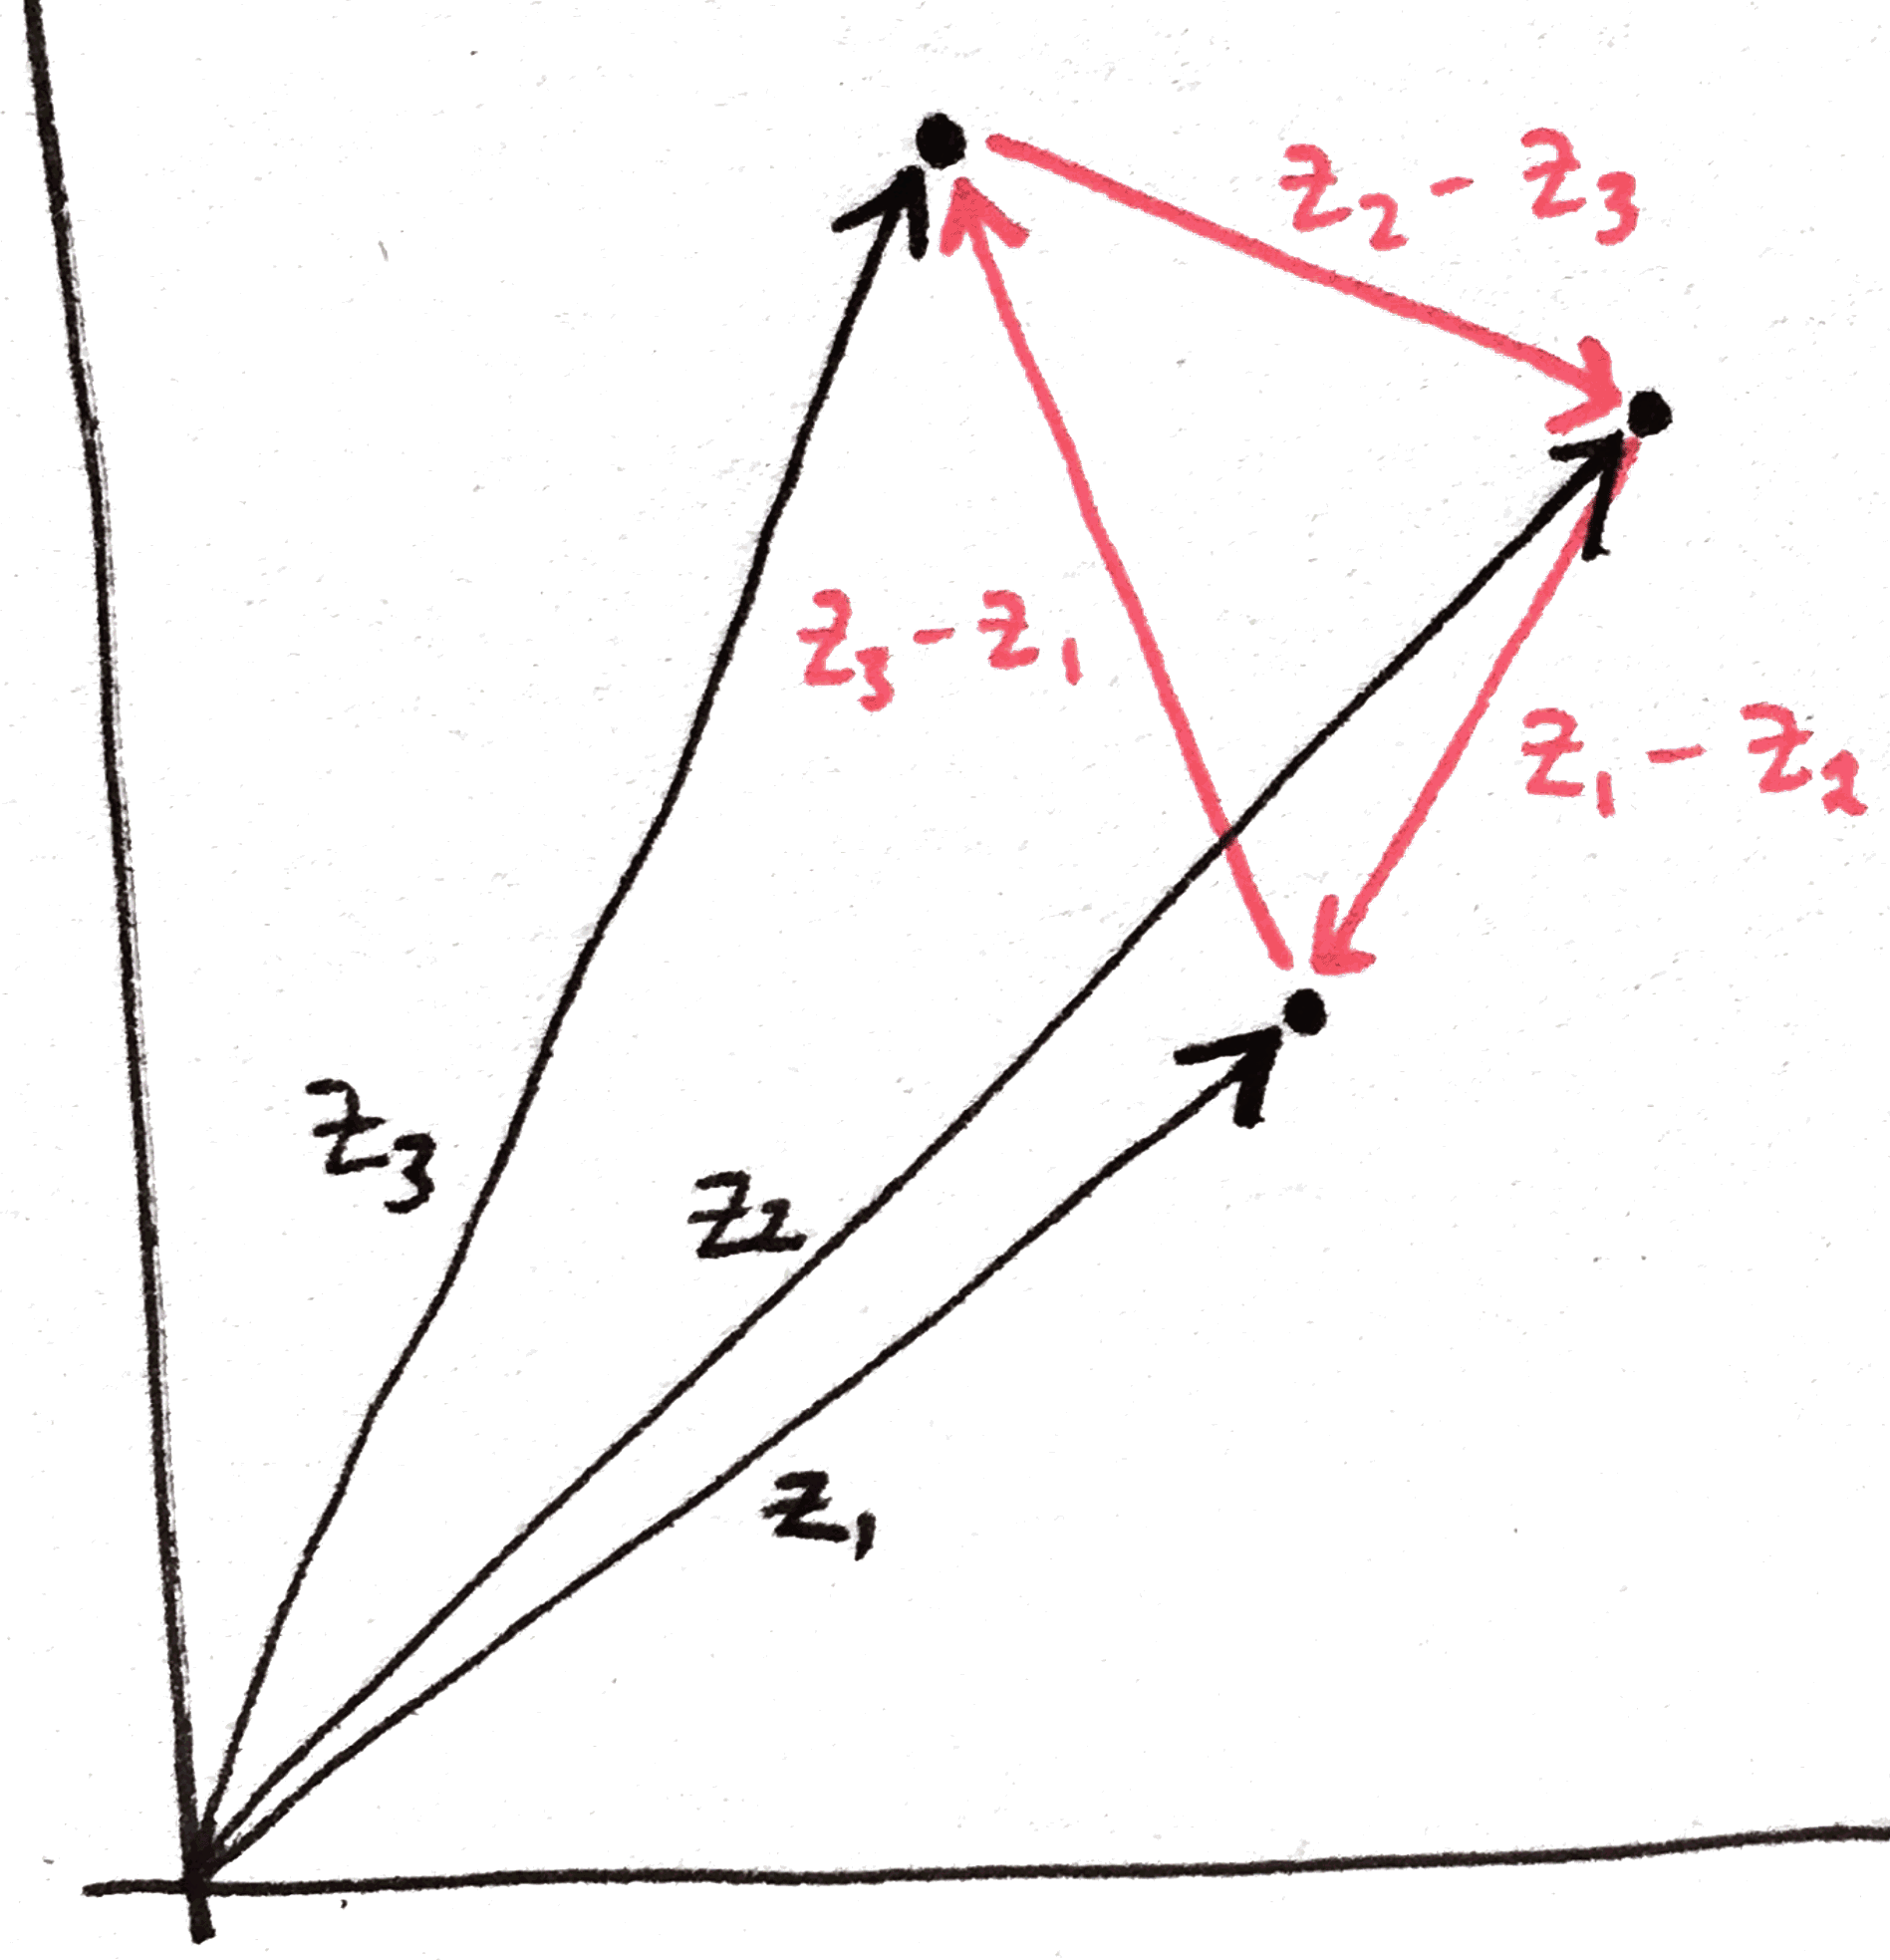
\includegraphics[width=100pt]{img/equilateral-1.png}

%   So the original claim is equivalent to the claim that the three vectors
%   $$
%   (z_1 - z_2)^2, ~ (z_2 - z_3)^2, ~ (z_3 - z_1)^2
%   $$
%   sum to 0 if and only if the triangle is equilateral.

%   First let's prove that if the triangle is equilateral, then the three vectors
%   sum to 0. Translate each of the unsquared vectors
%   $$
%   (z_1 - z_2), ~ (z_2 - z_3), ~ (z_3 - z_1)
%   $$
%   so that they originate at the origin; they are of equal magnitude and they
%   divide the circle into 3 sectors of equal angle $\frac{2\pi}{3}$. Let
%   $\theta < \frac{2\pi}{3}$ be the arbitrary angle between one of the vectors and
%   the first coordinate axis. Interpreted as complex numbers, we see that their
%   arguments are $\theta$, $\frac{2\pi}{3} + \theta$, and
%   $\frac{4\pi}{3} + \theta$.

%   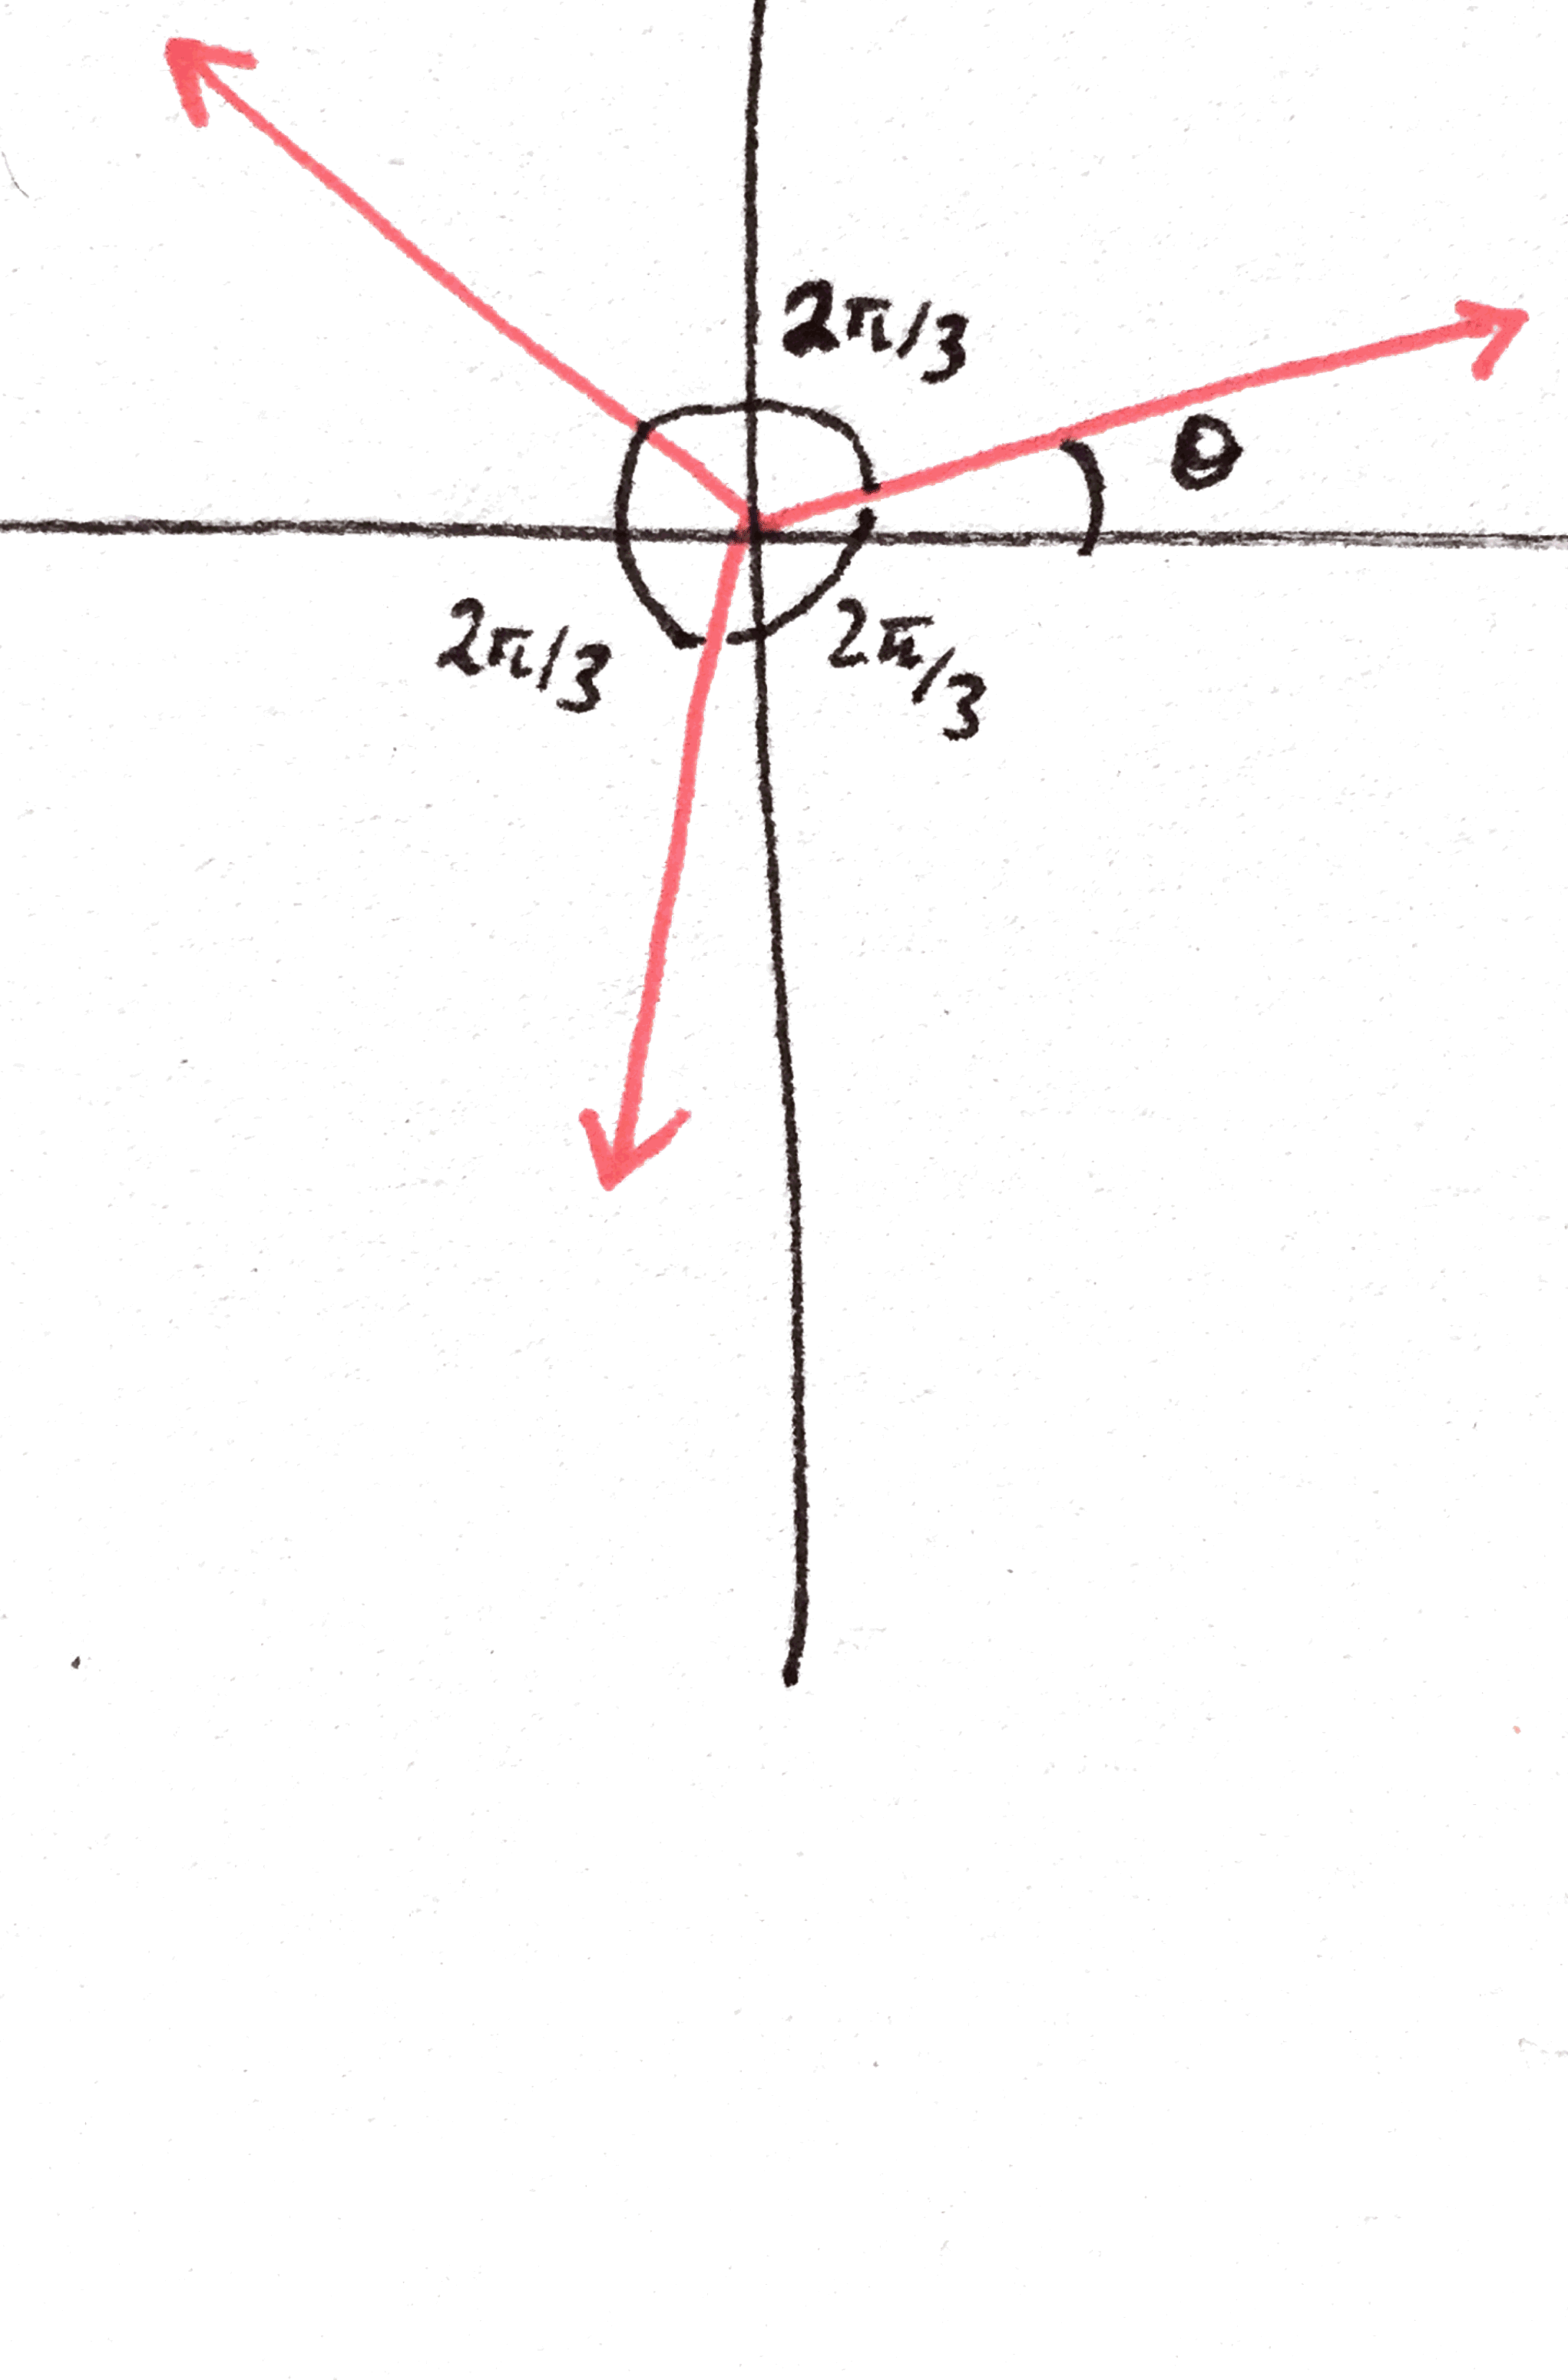
\includegraphics[width=100pt]{img/equilateral-2.png}

%   Now we form their squares
%   $$
%   (z_1 - z_2)^2, ~ (z_2 - z_3)^2, ~ (z_3 - z_1)^2.
%   $$
%   Since $(z_1 - z_2)$, $(z_2 - z_3)$, and $(z_3 - z_1)$ are of equal magnitude,
%   so are their squares. And the arguments of their squares are $2\theta$,
%   $\frac{4\pi}{3} + 2\theta$, and
%   $\frac{8\pi}{3} + 2\theta \equiv \frac{2\pi}{3} + 2\theta$ mod
%   $2\pi$. Therefore the three squared side vectors, when translated so that
%   they originate at the origin, also divide up the circle into sectors of equal
%   angle $\frac{2\pi}{3}$: the geometrical picture differs from the previous one
%   only by a uniform scaling and relabeling of the vectors, and we conclude that
%   these squared vectors also sum to zero (return to the origin when placed
%   head-to-tail). I.e. the equilaterality assumption implies
%   $$
%   (z_1 - z_2)^2 + (z_2 - z_3)^2 + (z_3 - z_1)^2 = 0,
%   $$
%   proving one direction of the equivalence.

%   To prove the other direction, we need to show that if
%   $$
%   z_1^2 + z_2^2 + z_3^2 = z_1z_2 + z_2z_3 + z_3z_1,
%   $$
%   or equivalently,
%   $$
%   (z_1 - z_2)^2 + (z_2 - z_3)^2 + (z_3 - z_1)^2 = 0,
%   $$
%   then the triangle is equilateral. For example, it would suffice to show that
%   $$
%   |z_1 - z_2| = |z_2 - z_3| = |z_3 - z_1|,
%   $$
%   but I haven't found a way to do so.

%   % The left side of this equation obeys the following triangle inequality
%   % $$
%   % |z_1^2 + z_2^2 + z_3^2|
%   % \le |z_1|^2 + |z_2|^2 + |z_3|^2,
%   % $$
%   % and the right side obeys
%   % $$
%   % |z_1z_2 + z_2z_3 + z_3z_1|
%   % \le |z_1||z_2| + |z_2||z_3| + |z_3||z_1|.
%   % $$

% \exercise{I.10.1}{Use de Moivre's formula to find expressions for
%   $\cos 5\theta$ and $\sin 5\theta$ as polynomials in $\cos \theta$ and
%   $\sin \theta$.}

%   From de Moivre's formula we have
%   $(\cos\theta + i\sin\theta)^5 = \cos 5\theta + i\sin 5\theta$. The left hand
%   side expands as
%   \begin{align*}
%   (\cos\theta + i\sin\theta)^5 =& \cos^5\theta \\
%                                &+ 5i\cos^4\theta\sin\theta \\
%                                &- 10\cos^3\theta\sin^2\theta \\
%                                &- 10i\cos^2\theta\sin^3\theta \\
%                                &+ 5\cos\theta\sin^4\theta \\
%                                &+ i\sin^5\theta.
%   \end{align*}
%   Equating real and imaginary components from the right side and the expansion of
%   the left side we have
%   \begin{align*}
%   \cos 5\theta &= \cos^5\theta - 10\cos^3\theta\sin^2\theta + 5\cos\theta\sin^4\theta \\
%   \sin 5\theta &= \sin^5\theta - 10\cos^2\theta\sin^3\theta + 5\cos^4\theta\sin\theta
%   \end{align*}
%   We can write these as polynomials in $\cos\theta$ and $\sin\theta$
%   respectively by using the identity $\cos^2\theta = 1 - \sin^2\theta$:
%   \begin{align*}
%   \cos 5\theta
%   &= \cos^5\theta - 10\cos^3\theta(1 - \cos^2\theta) + 5\cos\theta(1 - 2\cos^2\theta + \cos^4\theta) \\
%   &= 16\cos^5\theta - 20\cos^3\theta + 5\cos\theta, \\
%   \sin 5\theta
%   &= \sin^5\theta - 10(1 - \sin^2\theta)\sin^3\theta + 5(1 - 2\sin^2\theta + \sin^4\theta)\sin\theta \\
%   &= 16\sin^5\theta - 20\sin^3\theta + 5\sin\theta.
%   \end{align*}

% \exercise{I.11.4}{Prove that the sum of the $n$-th roots of 1 equals 0,
%   ($n > 1$).}

% Let $w = \cos \frac{2\pi}{n} + i\sin \frac{2\pi}{n}$ be the $n$-th root of 1
% with smallest argument, other than 1 itself. Then the sum of the roots is
% $1 + w + w^2 + \ldots + w^{n-1}$. This is the first $n$ terms of a geometric
% series with constant ratio $w$, and is therefore equal to
% $\frac{1 - w^{n}}{1 - w} = \frac{1 - 1}{1 - w} = 0$.


% \exercise{I.11.5}{Let $w$ be an $n$-th root of 1 different from 1
%   itself. Establish the formulas
%   $$
%   1 + 2w + 3w^2 + \ldots + nw^{n-1} = \frac{n}{w -1},
%   $$
%   $$
%   1 + 4w + 9w^2 + \ldots + n^2w^{n-1} = \frac{n^2}{w-1} - \frac{2n}{(w-1)^2}.
%   $$
% }

%   [Note: my answers to this question appear to be wrong.]

%   The sum of the first $n+1$ terms of a geometric series with first term $1$ and
%   constant ratio $w$ is

%   $$
%   1 + w + w^2 + \ldots + w^{n} = \frac{~~~~~1 - w^{n+1}}{1 - w} = \frac{1 - w}{1 - w} = 1,
%   $$
%   since $w^{n+1} = w$.

%   \textcolor{red}{This equation is true for $w$ in $n$-th root, but not for any $w$.}

%   Taking derivatives of both sides gives
%   $$
%   1 + 2w + 3w^2 + \ldots + nw^{n-1} = 0,
%   $$

%   which does not agree with the given formula, so something's wrong.

%   \textcolor{red}{To take derivatives of both sides need to write a function
%     identity, not an identity between two numbers.}

%   Nevertheless, if it were the case that
%   $$
%   1 + 2w + 3w^2 + \ldots + nw^{n-1} = \frac{n}{w -1}
%   $$
%   then we could multiply by $w$, giving
%   $$
%   w + 2w^2 + 3w^3 + \ldots + nw^n = \frac{nw}{w -1},
%   $$
%   and differentiate with respect to $w$ again, giving
%   $$
%   1 + 4w + 9w^2 + \ldots + n^2w^{n-1} = \frac{(w-1)n - nw}{(w - 1)^2} = \frac{n}{w - 1} - \frac{nw}{(w - 1)^2},
%   $$
%   which also doesn't agree with the given formula.

%   \textcolor{red}{Again, to take a derivative, need a function on RHS that
%     agrees with LHS $\forall w$.}

% % \begin{comment}

% \exercise{I.13.1}{Stereographic projection}

%   The stereographic projection maps $z$ onto the surface of a sphere according to
%   $$
%   z \mapsto \frac{(2 \Re z, 2 \Im z, |z|^2 - 1)}{|z|^2 + 1}.
%   $$
%   % It's 1-1 and the inverse map is
%   % $$
%   % (\xi, \eta, \zeta) \mapsto (s + 1)\frac{\xi}{2} + (s + 1)\frac{\eta}{2}i
%   % $$

% \exercise{I.13.1}{Establish the following formula for the spherical metric
% $$
% \rho(z_1, z_2) = \frac{2|z_1 - z_2|}{\sqrt{|z_1|^2 + 1}\sqrt{|z_2|^2 + 1}}
% $$}

%   $\rho(z_1, z_2)$
%   is the Euclidean distance between the image points of $z_1$ and $z_2$ on the
%   Riemann sphere, therefore
%   \begin{align*}
%   \rho(z_1, z_2)
%   &=
%   \left|
%   \frac{(2 \Re z_1, 2 \Im z_1, |z_1|^2 - 1)}{|z_1|^2 + 1} -
%   \frac{(2 \Re z_2, 2 \Im z_2, |z_2|^2 - 1)}{|z_2|^2 + 1}
%   \right| \\
%   &=
%   \left|
%   \frac{
%   (2 \Re z_1, 2 \Im z_1, |z_1|^2 - 1)(|z_2|^2 + 1) -
%   (2 \Re z_2, 2 \Im z_2, |z_2|^2 - 1)(|z_1|^2 + 1)
%   }
%   {(|z_1|^2 + 1)(|z_2|^2 + 1)}
%   \right| \\
%   \end{align*}
%   Meanwhile,
%   $$
%   |z_1 - z_2| = \sqrt{(\Re z_1 - \Re z_2)^2 + (\Im z_1 - \Im z_2)^2}
%   $$

% % \end{comment}

% \exercise{I.14.1}{Establish the formula
% $$
% \rho(z, \infty) = \frac{2}{\sqrt{|z|^2 + 1}}
% $$
% }

%   $\rho(z, \infty)$ is the Euclidean distance between the image point of $z$ and
%   the north pole $(0, 0, 1)$:
%   \begin{align*}
%   \rho(z, \infty)
%   &= \sqrt{
%   \(\frac{2 \Re z}{|z|^2 + 1} - 0\)^2 +
%   \(\frac{2 \Im z}{|z|^2 + 1} - 0\)^2 +
%   \(\frac{|z|^2 - 1}{|z|^2 + 1} - 1\)^2
%   } \\
%   &= \frac
%   {\sqrt{4 \(\Re z\)^2 + 4 \(\Im z\)^2 + 4}}
%   {|z|^2 + 1} \\
%   &= \frac
%   {2}
%   {\sqrt{|z|^2 + 1}}.
%   \end{align*}

% \end{description}

% \section*{II. Complex Differentiation}

% Consider $z$ approaching $z_0$. $z - z_0$ is a vector pointing from $z_0$ to
% $z$, and $f(z) - f(z_0)$ is a vector pointing between the image points for some
% complex-valued function $f$. The derivative of $f$ at $z_0$ is the rotation +
% scaling linear transformation (i.e. the complex number $c$) that takes
% $z - z_0$ as close as possible to $f(z) - f(z_0)$. Note that the transformation
% must be the \textit{same} regardless of the path taken by $z$ as it approaches
% $z_0$. In other words, the action of $f$ on \textit{all} vectors in an
% infinitisimal disc around $z_0$ is the same as multiplying by a complex number
% $c$.

% The transformation $f$ can be described by two surfaces over the complex plane:
% $u(x,y)$ and $v(x,y)$, so that $f: \cvec{x}{y} \mapsto
% \cvec{u(x,y)}{v(x,y)}$. If $f$ is differentiable at $(x_0, y_0)$ then it has a
% local linear approximation with sublinear error. That linear approximation is
% $$
% \cvec{u(x, y)}
%      {v(x, y)} \approx \cvec{u(x_0, y_0)}
%                             {v(x_0, y_0)} + \cvec{(x - x_0)\dudx + (y - y_0)\dudy}
%                                                  {(x - x_0)\dvdx + (y - y_0)\dvdy}
% $$
% This is more succinctly expressed using the Jacobian:
% $$
% \cvec{u(x, y)}
%      {v(x, y)} \approx \cvec{u(x_0, y_0)}
%                             {v(x_0, y_0)} + \mat{u_x}{u_y}
%                                                 {v_x}{v_y} \cvec{x - x_0}
%                                                                 {y - y_0}.
% $$
% Note that this "linear approximation" form
% $$
% y \approx y_0 + y'(x - x_0)
% $$
% could just as well be written
% $$
% y - y_0 \approx y'(x - x_0)
% $$
% showing that one way of describing the derivative is "whatever you have to
% multiply a small displacement in the input space by to get the displacement in
% the output space".

% Recall that the derivative of a complex function $f$ is defined to be a complex
% number,
% $$
% f'\(\cvec{x_0}
%         {y_0}\) = \lim_{(x,y) \rightarrow (x_0,y_0)}
% \frac{
% \cvec{u(x, y)}
%      {v(x, y)} - \cvec{u(x_0)}
%                       {v(y_0)}
% }
% {
% \cvec{x}
%      {y} - \cvec{x_0}
%                 {y_o}.
% },
% $$
% i.e.
% $$
% f'(z_0) = \lim_{z \rightarrow z_0} \frac{f(z) - f(z_0)}{z - z_0},
% $$
% i.e. the derivative is whatever complex number you multiply the vector $z-z_0$
% by to get its image vector $f(z) - f(z_0)$, in the limit as $z \rightarrow z_0$.

% The partial derivatives of the complex-valued $f$ in the real and imaginary
% directions are the complex numbers
% \begin{align*}
% f_x &= u_x + iv_x\\
% f_y &= u_y + iv_y\\
% \end{align*}
% or
% \begin{align*}
% f_x &= \cvec{u_x}{v_x}\\
% f_y &= \cvec{u_y}{v_y}\\
% \end{align*}

% The geometric interpretation of these is that they define how the image vector
% $f(z)$ changes in response to a small change to $z$.

% $u$ can be approximated by a local tangent plane. That's what $u_x$ and $u_y$
% do. And so can $v$; that's what $v_x$ and $v_y$ do. But when we consider the
% effect of a small displacement in the 2D input space on the 2D output space, we
% describe the two tangent plane approximations jointly as a linear
% transformation of the input plane, defined by the Jacobian. The thing is, the
% linear transformation must have the same effect as multiplication by a complex
% number.

% The derivative is "what you have to multiply the input displacement by to get
% the output displacement". That's true for a single-variable function
% $\R \rightarrow \R$
% $$
% u(x) - u(x_0) = f'(x_0) \cdot (x - x_0)
% $$
% and it's true for a surface over the plane $(\R^2 \rightarrow \R$)
% $$
% u(x, y) - u(x_0, y_0) = \dudx \cdot (x - x_0) + \dudy \cdot (y - y_0)
% $$
% so presumably something analogous holds for a linear transformation of the
% plane $(\R^2 \rightarrow \R^2$), i.e.
% $$
% \vec z - \vec z_0 = \dveczdx \cdot (x - x_0) + \dveczdy \cdot (y - y_0).
% $$
% or
% $$
% \cvec{u(x, y)}{v(x, y)} - \cvec{u(x_0, y_o)}{v(x_0, y_0)} =
% \cvec{u_x}{v_x} \cdot (x - x_0) + \cvec{u_y}{v_y} \cdot (y - y_0).
% $$
% That's exactly the same as the equation involving the Jacobian above
% $$
% \cvec{u(x, y)}
%      {v(x, y)} - \cvec{u(x_0, y_0)}
%                       {v(x_0, y_0)} = \mat{u_x}{u_y}
%                                           {v_x}{v_y} \cvec{x - x_0}
%                                                           {y - y_0}.
% $$

% So how are we to make sense of the equation relating $f'$ and the partial
% derivatives $\dfdx$ and $\dfdy$? Clearly in some sense the Jacobian \textit{is}
% $f'$, or at least, the complex number that does what the Jacobian does is
% $f'$. And
% \begin{align*}
% \dfdx &= \cvec{u_x}
%               {v_x} = u_x + iv_x \\
% \dfdy &= \cvec{u_y}
%               {v_y} = u_y + iv_y,
% \end{align*}
% and so from the Cauchy-Riemann constraint
% \begin{align*}
% \dfdy &= -v_x + iu_x = i\dfdx,
% \end{align*}
% i.e. the partial derivative w.r.t. $y$ points at 90° to the $x$ partial
% derivative.

% % $f_x$ is the complex number that transforms a small real displacement vector
% % $\epsilon$ to its image, and $f_y$ is the complex number that transforms a
% % small imaginary displacement vector $i\delta$ to its image. [But shouldn't
% % these be the same and equal to $f'$, seeing as $f'$ rotates and scales all
% % displacement vectors in an infinitesimal disc uniformly? Instead, C-R says that
% % $f_x = -if_y$.]

% % One notation for the "directional derivative" of $f$ in the direction of
% % $\vec z$ is $\frac{\partial f}{\partial \vec z}$. Is this an entirely separate
% % notion from the partial derivatives $\frac{\partial f}{\partial z}$ and
% % $\frac{\partial f}{\partial \bar z}$ considered in the context of complex
% % analysis / Wirtinger derivatives?

% So if the local linear approximation to the transformation $f$ behaves exactly as
% multiplication by a complex number, then the Jacobian must have the form of a
% rotation+scale matrix, $\smat{a}{-b}
%                              {b}{a}$. Therefore the Jacobian must satisfy the
% Cauchy-Riemann equations
% $$
% \begin{cases}
% u_x = v_y \\
% v_x = -u_y. \\
% \end{cases}
% $$
% The Jacobian that effects the local linear rotation+scale transformation, together with
% the equivalent complex number, is
% $$
% \mat{u_x}{-v_x}
%     {v_x}{u_x} ~~~~ u_x + iv_x
% $$
% or
% $$
% \mat{v_y}{u_y}
%     {-u_y}{v_y} ~~~~ v_y - iu_y.
% $$
% So we can write
% \begin{align*}
% f'
% &= u_x + iv_x = f_x \\
% &= v_y - iu_y = -if_y,
% \end{align*}
% therefore as above, another expression of the Cauchy-Riemann criterion is
% $$
% f_x = -if_y.
% $$
% Question: what is the intuition for the fact that the complex number
% representing the partial derivative with respect to $x$ is the \textit{same} as
% the complex number that effects the full linear transformation? (and at 90° to
% the partial with respect to $y$) And what's the intuition for the fact that
% $\dfdz = \dfdx$, while $\dfdzbar = 0$?

% % The partial derivatives of the complex-valued $f$ in the real and imaginary
% % directions are
% % \begin{align*}
% % \dfdx &= \dudx + i\dvdx\\
% % \dfdy &= \dudy + i\dvdy\\
% % \end{align*}

% % So we can write
% % \begin{align*}
% % f'(z_0)
% % &= \dudx(z_0) + i \dvdx(z_0) =   \dfdx(z_0) \\
% % &= \dvdy(z_0) - i \dudy(z_0) = -i\dfdy(z_0),
% % \end{align*}
% % or
% % \begin{align*}
% % f'\(\cvec{x_0}{y_0}\)
% % &= \cvec{\dudx(z_0)}{\dvdx(z_0)}  =   \dfdx(z_0)  \\\\
% % &= \cvec{\dvdy(z_0)}{-\dudy(z_0)} = -i\dfdy(z_0).
% % \end{align*}

% $f$ is differentiable iff the error in the linear transformation goes to $0$ as
% $(x,y) \rightarrow (x_0,y_0)$ (i.e. real partial derivatives of $u$ and $v$
% exist) and the partial derivatives satisfy the Cauchy-Riemann equations.

% \subsection*{Partial derivatives in the $z$ and $\bar z$ directions}
% The (fixed) $x, y$ and (varying) $z, \bar z$ directions are related by
% \begin{align*}
% x &= (z + \bar z)/2 \\
% y &= (z - \bar z)/2i.
% \end{align*}
% So by the chain rule,
% \begin{align*}
% \dfdz
% &= \dfdx \dxdz + \dfdy \dydz \\
% &= (u_x + iv_x)\frac{1}{2} + i(u_x + iv_x)\frac{1}{2i} \\
% &= u_x + iv_x \\
% &= \dfdx
% \end{align*}
% and
% \begin{align*}
% \dfdzbar
% &= \dfdx \dxdzbar + \dfdy \dydzbar \\
% &= (u_x + iv_x)\frac{1}{2} + i(u_x + iv_x)\frac{-1}{2i} \\
% &= \frac{1}{2}\Big((u_x - u_x) + i(v_x - v_x)\Big) \\
% &= 0.
% \end{align*}

% \begin{description}

% \exercise{II.8.1(b,d)}{
%   Let the function $f$ be holomorphic in the open disc $D$. Prove that each of
%   the following conditions forces $f$ to be constant:\\\\
%   \textnormal{Let $f(z) = u(z) + iv(z)$.}
%   \begin{description}
%     \exercise{(a)}{$f' = 0$ throughout $D$} \\\\
%     \textnormal{ \textbfit{Informally:} $f' = 0$ throughout $D$ means that the
%       best linear approximation of $f(z) - f(z_0)$ is $0(z - z_0)$ which
%       implies that $f(z) = f(z_0)$ everywhere, so $f$ is constant.\\
%       ~\\
%       \textbfit{Formally:} Since $f$ is holomorphic, $f' = u_x + iv_x =
%       0$. Equating real and imaginary parts shows that $u_x = v_x = 0$ and
%       therefore that $v_y = u_x = 0$ and $u_y = -v_x = 0$. Since the Jacobian
%       of $f$ is the zero matrix, $f$ is constant.}\\
%     \exercise{(b)}{$f$ is real-valued in $D$} \\\\
%     \textnormal{
%       % \textbfit{Informally:}
%       $f$ is real-valued, so $f(z) - f(z_0)$ is real-valued. Therefore the
%       local linear approximation $c(z - z_0)$ collapses the plane onto the real
%       axis, i.e. the Jacobian matrix has the form $\mat{a}{b} {0}{0}$. But $f$
%       is holomorphic, so the Jacobian must also have the form
%       $\mat{a}{-b}
%            {b}{a}$. Therefore the Jacobian is the zero matrix, i.e.
%       all partial derivatives are zero, $u_x = u_y = v_x = v_y = 0$, so $f$ is constant.\\
%       % \textbfit{Formally:} $f$ is real-valued means that $v(z) = 0$
%       % everywhere. Therefore the partial derivatives $v_x = v_y = 0$. Since $f$
%       % is holomorphic the partial derivatives satisfy the Cauchy-Riemann
%       % equations, therefore we have $u_x = v_y = 0$ and $u_y = -v_x = 0$. The
%       % Jacobian is the zero matrix hence $f$ is constant.
%       % \\
%     }
%     \exercise{(c)}{$|f|$ is constant in $D$} \\\\
%     \textnormal{ \textbfit{Informally:} $|f|$ is constant means that it collapses
%       all points in the open disc $D$ onto a circle. Therefore the Jacobian of
%       $f$ has determinant $0 = u_x^2 + v_x^2 = v_y^2 + u_y^2$. Therefore the
%       Jacobian
%       is the zero matrix and the function $f$ is constant.\\
%       ~\\
%       \textbfit{Formally:} $|f|$ is constant, therefore
%       $|f|^2 = f\bar f = u^2 + v^2$ is constant. Therefore the following two
%       partial derivatives are constant:
%       \begin{align*}
%         \begin{cases}
%           \ddx |f|^2 =  2uu_x + 2vv_x = 0 \\
%           \ddy |f|^2 = 2uu_y + 2vv_y = 0.
%         \end{cases}
%       \end{align*}
%       Since $f$ is holomorphic, $u_x = v_y$ and $u_y = -v_x$, so
%       \begin{align*}
%         \begin{cases}
%           uu_x - vu_y = 0 \\
%           uu_y + vu_x = 0,
%         \end{cases}
%       \end{align*}
%       % i.e.
%       % $$
%       % \mat{u}{-v}
%       %     {u}{v} \cvec{u_x}{u_y} = \cvec{0}{0}.
%       % $$
%       % The determinant of this system is $2uv$ which is not in general zero. But
%       % the equations hold throughout the disc $D$, therefore
%       Multiplying the first equation by $u$ and the second by $v$ we have
%       $$
%       \begin{cases}
%         u^2u_x - uvu_y = 0 \\
%         uvu_y + v^2u_x = 0,
%       \end{cases}
%       $$
%       and summing these gives
%       $$
%       u_x(u^2 + v^2) = 0,
%       $$
%       which proves that either $u_x = 0$ or that $f$ is constant (in which case $u_x = 0$ also).\\
%       Similarly, multiplying the first equation by $v$ and the second by $u$ gives
%       $$
%       \begin{cases}
%         uvu_x - v^2u_y = 0 \\
%         u^2u_y + uvu_x = 0,
%       \end{cases}
%       $$
%       and subtracting the first from the second gives
%       $$
%       u_y(u^2 + v^2) = 0.
%       $$
%       We conclude that $u_x = u_y = 0$ and that $f$ is therefore constant.  }
%     \exercise{(d)}{$\arg f$ is constant in $D$} \\\\
%     \textnormal{
%       %\textbfit{Informally:}
%       Let $\arg f = \theta$, constant throughout
%       $D$. Then $\arg (f(z) - f(z_0)) = \theta$, whenever $z \neq z_0$.
%       Therefore the best local linear approximation to $f$ is a linear
%       transformation that collapses the plane onto a line with angle $\theta$.
%       The Jacobian determinant is therefore zero. Since $f$
%       is holomorphic the Jacobian is of the form $\mat{a}{-b}
%                                                       {b}{a}$ and therefore we have
%       $a^2 + b^2 = 0$, so $a = b = 0$.  Therefore the Jacobian is the zero
%       matrix, i.e. $f' = 0$ throughout $D$, so $f$ is constant.\\
%       % ~\\
%       % \textbfit{Formally:}
%       % The polar form of the Cauchy-Riemann equations is
%       % \begin{align*}
%       % v_\theta &= ru_r \\
%       % u_\theta &= -rv_r.
%       % \end{align*}
%       % Since $\arg f$ is constant, $v_\theta$
%     }
%   \end{description}
% }

% \exercise{II.8.2}{
%   Let the function $f$ be holomorphic in the open set $G$. Prove that the
%   function $g(z) = \bar{f(\bar z)}$ is holomorphic in the set
%   $G^* = \{\bar z: z \in G\}$.
% } \\\\
% Let
% \begin{align*}
% f: x + iy &\mapsto s(x, y) + i t(x,y). \\
% g: x + iy &\mapsto u(x, y) + i v(x,y) \\
% \end{align*}
% We want to show that the Jacobian of $g$ exists and and satisfies the
% Cauchy-Riemann equations. We have
% \begin{align*}
% g(x + iy)
% &= \bar{s(x, -y) + i t(x, -y)} \\
% &= s(x, -y) - i t(x, -y),
% \end{align*}
% and therefore
% \begin{align*}
%   u(x,y) &= s(x, -y) \\
%   v(x, y) &= -t(x, -y).
% \end{align*}
% Now $f = s + it$ is holomorphic, so $s_x=t_y$ and $s_y = -t_x$. Therefore the
% partial derivatives of $g$ are
% \begin{align*}
%   u_x &= \ddx s(x, -y)  = s_x \\
%   u_y &= \ddy s(x, -y)  = -s_y = t_x \\
%   v_x &= -\ddx t(x, -y) = -t_x \\
%   v_y &= -\ddy t(x, -y) = t_y = s_x. \\
% \end{align*}
% Therefore $u_x = v_y$ and $v_x = -u_y$, showing that the Jacobian of $g$
% satisfies the Cauchy-Riemann equations, and therefore that $g$ is holomorphic
% in its domain.

% \exercise{II.16.4}{
%   Prove that, if $u$ is a real-valued harmonic function in an open disk $D$,
%   then any two harmonic conjugates of $u$ in $D$ differ by a constant.
% }

% Let $v$ and $w$ be harmonic conjugates of $u$, so that
% $$
% \begin{cases}
% u_x = v_y = w_y\\
% u_y = -v_x = -w_x.
% \end{cases}
% $$
% We want to show that $q = v-w$ is constant, i.e. that $q_x = q_y = 0$,
% throughout $D$. From the Cauchy-Riemann equalities above, we have
% $q_x = v_x - w_x = 0$ and $q_y = v_y - w_y = 0$ as required.

% % \exercise{II.16.5}{
% %   [Not in homework.] Suppose that $u$ is a real-valued harmonic function in an open disk $D$, and
% %   suppose that $u^2$ is also harmonic. Prove that $u$ is constant.
% % }

% \exercise{II.16.7}{
%   Prove (assuming equality of second-order mixed partial derivatives) that
%   $$
%   \dddzbarz =
%   \frac{1}{4}\(\frac{\partial^2}{\partial x^2} +
%                \frac{\partial^2}{\partial y^2}\)
%   $$
%   Thus, Laplace's equation can be written as $\frac{\partial^2 f}{\partial \bar z \partial z} = 0$.
% }

% First note that $x$ and $y$ are related to $\bar z$ via
% \begin{align*}
% x = \frac{z + \bar z}{2} \\
% y = \frac{z - \bar z}{2i}, \\
% \end{align*}
% therefore by the chain rule
% \begin{align*}
% \dzbar
% &= \ddx \dxdzbar = \frac{1}{2}\ddx \\
% &= \ddy \dydzbar = -\frac{1}{2i}\ddy. \\
% \end{align*}

% Now $\ddz$ is defined by
% $$
% \ddz = \frac{1}{2}\(\ddx - i\ddy\),
% $$
% and taking the partial derivative with respect to $\bar z$ gives
% \begin{align*}
% \dddzbarz
% &= \frac{1}{2}\(\dzbar \ddx - i \dzbar \ddy\) \\
% &= \frac{1}{2}\(\frac{1}{2}\ddx \ddx - i \(\frac{-1}{2i}\)\ddy \ddy\) \\
% &= \frac{1}{4}\(\dddxx + \dddyy\).
% \end{align*}

% Laplace's equation is $\ddfdxx + \ddfdyy = 0$, which can also be written as
% $$
% \(\dddxx + \dddyy\)f = 0,
% $$
% and therefore
% $$
% 4 \dddzbarz f = 0,
% $$
% i.e.
% $$
% \dddfzbarz = 0.
% $$

% \exercise{II.16.8}{
%   Prove that if $u$ is a real-valued harmonic function then the function
%   $\frac{\partial u}{\partial z}$ is holomorphic.
% }
% As above, first note that $x$ and $y$ are related to $\bar z$ via
% \begin{align*}
% x &= \frac{z + \bar z}{2} \\
% y &= \frac{z - \bar z}{2i} = -i\frac{z - \bar z}{2}. \\
% \end{align*}
% By the chain rule
% \begin{align*}
% \dudz
% &= \dudx \dxdz + \dudy \dydz \\
% &= \frac{1}{2} \dudx  - \frac{i}{2} \dudy. \\
% \end{align*}
% Switching notation, we write this as $\dudz = \frac{1}{2} u_x  - \frac{i}{2} u_y$.

% Define a complex-valued function
% \begin{align*}
% w(x + iy)
% = \dudz &= s(x,y) + it(x,y) \\
% &= \frac{1}{2} u_x  - \frac{i}{2} u_y.
% \end{align*}
% Then the Jacobian of $w$ is
% \begin{align*}
% \mat{s_x}{s_y}
%     {t_x}{t_y} = \frac{1}{2}\mat{u_{xx}}{u_{xy}}
%                                 {-u_{yx}}{-u_{yy}}.
% \end{align*}
% But since $u$ is harmonic, we know that $u_{xx} + u_{yy} = 0$, therefore the
% Jacobian of $w$ satisfies the Cauchy-Riemann equations and $w = \dudz$ is
% holomorphic.

% \end{description}

% \section*{Image of a curve under a transformation}
% What is the effect of the inversion mapping $z \mapsto w = \frac{1}{z}$ on circles
% and lines?

% Let $z = x + iy$ with image $w = \frac{1}{z} = u + iv$ and note that
% $\frac{1}{z} = \frac{\bar z}{|z|^2}$. Therefore the mapping is
% \begin{align*}
%   x + iy \mapsto \frac{x}{x^2 + y^2} - i\frac{y}{x^2 + y^2} = u + iv.
% \end{align*}

% The general equation of a circle or line in the plane is
% \begin{align*}
%   Ax^2 + Ay^2 + Bx + Cy + D  = 0.
% \end{align*}

% We use the inverse mapping to establish an equation that holds in the
% transformed complex plane. Since the inverse mapping is the same as the forward
% mapping, we have
% \begin{align*}
%   w = u + iv \mapsto \frac{u}{u^2 + v^2} - i\frac{v}{u^2 + v^2} = x + iy.
% \end{align*}
% So points $w = u + iv$ in the transformed complex plane satisfy
% \begin{align*}
%   A\frac{u^2}{(u^2 + v^2)^2} + A\frac{v^2}{(u^2 + v^2)^2} + B\frac{u}{u^2 + v^2} - C\frac{v}{u^2 + v^2} + D  = 0,
% \end{align*}
% i.e.
% \begin{align*}
%   \frac{A}{u^2 + v^2} + B\frac{u}{u^2 + v^2} - C\frac{v}{u^2 + v^2} + D  = 0,
% \end{align*}
% or
% \begin{align*}
%   A + Bu - Cv + Du^2 + Dv^2  = 0.
% \end{align*}
% So we see that, if a circle/line exists in the pre-transformed plane, then...



% \section*{III. Linear-Fractional Transformations}

% Complex projective space $\CP^1$ is a space of equivalence classes of vectors
% in $\C^2$. Basically the elements of $\CP^1$ are analogs of lines through the
% origin in $\R^2$ (one-dimensionsal subspaces): two vectors are equivalent if
% the ratios between their vector components are equal. And that ratio provides a
% bijection between $\CP^1$ and $\bar \C$.

% Since linear transformations of $\C^2$ map lines (in $\C^2$) to lines (in
% $\C^2$), they induce a bijection on $\CP^1$ and therefore on $\bar \C$.

% In fact linear-fractional transformations are induced by a two-by-two complex
% matrix (an element of $\GLC{2}$) [Do I understand why?]. This makes
% linear-fractional transformations closed under composition and gives them an
% identity (the LFT corresponding to the identity matrix) and inverses (given by
% the matrix inverse). So there is a group of LFTs which is the homomorphic image
% of $\GLC {2}$, under the map which sends a two-by-two matrix to its induced
% LFT. The kernel of the homomorphism contains scalar multiples of the identity
% matrix $I_2$. I think that's basically because such uniform scaling matrices
% leave lines unchanged and therefore leave the one-dimensional subspaces
% unchanged. Therefore the group of LFTs is isomorphic to the quotient group
% $\GLC{2}/(\C\backslash\{0\})I_2$ (each coset is formed by taking a matrix and
% scaling it by multipying it with a scaled identity matrix from the kernel).

% \begin{description}
%   \exercise{III.5.2}{
%     ~\\
%     Given four distinct points $z_1, z_2, z_3, z_4$ in $\bar \C$, their cross
%     ratio, which is denoted by $(z_1, z_2; z_3, z_4)$ is defined to be the
%     image of $z_4$ under the linear-fractional transformation that sends
%     $z_1,z_2,z_3$ to $\infty, 0, 1$, respectively. Prove that if $\phi$ is a
%     linear-fractional transformation then
%     $$\(\phi(z_1),\phi(z_2);\phi(z_3),\phi(z_4)\) = (z_1, z_2; z_3, z_4).$$
%     ~\\
%   }\\
%   Let $f$ be the linear-fractional transformation that maps $z_1, z_2, z_3$ to
%   $\infty, 0, 1$ respectively, so that the cross-ratio is defined to be
%   $(z_1, z_2; z_3, z_4) = f(z_4)$. We want to show that the cross ratio,
%   defined in this way, is invariant under an arbitrary linear-fractional
%   transformation $\phi$.

%   First, let's find an explicit expression for $f(z)$ in terms of
%   $z_1,z_2,z_3$. We know that $f(z_1) = \infty$ and $f(z_2) = 0$, so perhaps
%   $f$ has the form $f(z) = c\frac{z_2 - z}{z_1 - z}$ for some constant $c$. We
%   also require $f(z_3) = 1$. One way to achieve that is to choose
%   $c = \frac{z_1 - z_3}{z_2 - z_3}$, so the definition of $f$ becomes
%   $$
%   f(z) = c\frac{(z_2 - z)(z_1 - z_3)}{(z_2 - z_3)(z_1 - z)}.
%   $$
%   Defined like this, $f$ is a linear-fractional transformation, and it does
%   send $z_1,z_2,z_3$ to $\infty, 0, 1$, respectively. Furthermore, by theorem
%   III.5, this is the only linear-fractional transformation that does so.

%   So we have
%   $$
%   (z_1, z_2; z_3, z_4) = f(z_4) = \frac{(z_1 - z_3)(z_2 - z_4)}{(z_1 - z_4)(z_2 - z_3)},
%   $$
%   and we want to show that this quantity is invariant under an arbitrary
%   linear-fractional transformation $\phi$. Let
%   $\phi(z) = \frac{az + b}{cz + d}$, with $ad - bc = 1$ (since we are free to
%   scale the coefficients $a,b,c,d$ uniformly as we wish, if $ad - bc \ne 1$
%   then we scale them all by $\frac{1}{\sqrt{ad - bc}}$). Now consider
%   \begin{align*}
%     \phi(z_i) - \phi(z_j)
%     &= \frac{(az_i + b)(cz_j + d) - (az_j + b)(cz_i + d)}{(cz_i + d)(cz_j + d)} \\
%     &= \frac{z_iz_j(ac - ac) + z_i(ad - bc) + z_j(bc - ad) + (bd - bd)}{(cz_i + d)(cz_j + d)} \\
%     &= \frac{z_i - z_j}{(cz_i + d)(cz_j + d)}.
%   \end{align*}
%   Letting $A_i = cz_i + d$, we see that the cross-ratio of the transformed
%   points is
%   \begin{align*}
%     \(\phi(z_1),\phi(z_2);\phi(z_3),\phi(z_4)\) = \frac{(z_1 - z_3)(z_2 - z_4)/A_1A_3A_2A_4}{(z_1 - z_4)(z_2 - z_3)/A_1A_4A_2A_3} = (z_1, z_2; z_3, z_4).
%   \end{align*}

%   % $$
%   % z_1, z_2, z_3 = -\frac{d}{c}, \frac{b}{a}, \frac{+d - b}{-c + a}
%   % $$

%   \exercise{III.6.3}{
%     ~\\
%     Prove that a linear-fractional transformation with only one fixed point is
%     conjugate to a translation.
%     ~\\
%   }\\
%   Let $\phi(z) = \frac{az + b}{cz + d}$, with $ad - bc = 1$ (justified in
%   III.5.2 above). The fixed points of this mapping are the solutions of
%   \begin{align*}
%     \frac{az + b}{cz + d} = z,
%   \end{align*}
%   which is a quadratic equation
%   $$
%   cz^2 + (d - a)z - b = 0,
%   $$
%   with solutions
%   \begin{align*}
%   z &= \frac{(a - d) \pm \sqrt{(a - d)^2 + 4bc}}{2c} \\
%     &= \frac{(a - d) \pm \sqrt{(a + d)^2 - 4(ad - bc)}}{2c} \\
%     &= \frac{(a - d) \pm \sqrt{(a + d)^2 - 4}}{2c} \\
%   \end{align*}
%   $\phi_1$ has only one fixed point, so $a + d = \pm 2$, i.e. $d = 2 - a$ or $d = -2 - a$.

%   We want to show that there exists a linear-fractional transformation $\phi_2(z) = z + k$,
%   and another linear-fractional transformation $\psi$, such that
%   $\phi_2 = \psi \circ \phi_1 \circ \psi^{-1}$. In other words, performing the
%   $\phi_1$ transformation under the change of basis specified by $\psi$, yields
%   a translation.

%   Let's just try to show that by calculation. Let
%   $\psi(z) = \frac{ez + f}{gz + h}$ with $eh - fg = 1$ so that
%   $\psi^{-1}(z) = \frac{hz -f}{-gz + e}$. Then
%   \begin{align*}
%     \phi_2(z)
%     &= (\psi \circ \phi_1 \circ \psi^{-1})(z) \\
%     &= \mat{e}{f}
%            {g}{h} \mat{a}{b}
%                       {c}{d} \mat{h }{-f}
%                                  {-g}{e } \cvec{z}{1} \\
%     &= \mat{e}{f}
%            {g}{h} \mat{ ah - bg}{-af + be}
%                       {-ch - dg}{-cf + de} \cvec{z}{1} \\
%     &= \mat{e(ah - bg) + f(-ch - dg)}{e(-af + be) + f(-cf + de)}
%            {g(ah - bg) + h(-ch - dg)}{g(-af + be) + h(-cf + de)} \cvec{z}{1} \\
%   \end{align*}

%   Things we know:
%   \begin{itemize}
%   \item Trace is invariant under change of basis, so the trace of the product
%     of the 3 matrices is the same as that of $\phi_1$: $\pm 2$.
%   \item The determinants of all the matrices and products thereof are 1.
%   \end{itemize}
%   So
%   \begin{align*}
%     e(ah - bg) + f(-ch - dg) + g(-af + be) + h(-cf + de) &= \pm 2 \\
%     (ah - bg)(-cf + de) - (-af + be)(-ch - dg) &= 1 \\
%     eh - fg &= 1 \\
%     ad - bc &= 1 \\
%     a + d &= \pm 2
%   \end{align*}
%   A translation has matrix of the form $\mat{x}{y}
%                                             {0}{x}$. So the question is,
%   can we find $e,f,g,h$ such that
%   \begin{align*}
%     g(ah - bg) + h(-ch - dg) &= 0 \\
%     e(ah - bg) + f(-ch - dg) &= g(-af + be) + h(-cf + de)
%   \end{align*}

%   \begin{align*}
%     ah - bg = h(ch + dg)/g \\
%     eh(ch + dg)/g + f(-ch - dg) &= g(-af + be) + h(-cf + de)
%   \end{align*}

%   % \exercise{III.9.1}{
%   %   ~\\
%   %   Find the image of the half-plane $\Re z > 0$ under the linear-fractional
%   %   transformation that maps $0, i, -i$ to $1, -1, 0$, respectively.
%   %   ~\\
%   % }\\
%   % Let the linear-fractional transformation be $\phi(z) = \frac{az + b}{cz + d}$. We have
%   % \begin{align*}
%   %   \phi(-i) &= \frac{-ai + b}{-ci + d} = 0 \implies b = ai \\
%   %   \phi(0) &= \frac{b}{d} = 1 \implies d = b = ai \\
%   %   \phi(i) &= \frac{ai + b}{ci + d} = -1 \implies ci + d = -2b \implies c = -3a,
%   % \end{align*}
%   % so
%   % \begin{align*}
%   %   \phi(z) = \frac{az + ai}{-3az + ai} = \frac{z + i}{-3z + i}.
%   % \end{align*}
%   % % Now let's find how $z = x + iy$ is transformed:
%   % % \begin{align*}
%   % %   \phi(x + iy)
%   % %   &= \frac{x + iy + i}{-3(x + iy) + i} \\
%   % %   &= \frac{x + i(y + 1)}{-3x + i(-3y + 1)} \\
%   % %   &= \frac{(x + i(y + 1))(-3x - i(-3y + 1))}{9x^2 + (-3y + 1)^2} \\
%   % %   &= \frac{\Big(-3x^2 + (y + 1)(-3y + 1)\Big) + i\Big((y+1)(-3x) - x(-3y + 1)\Big)}{9x^2 + (-3y + 1)^2} \\
%   % %   &= \frac{\Big(-3x^2 + (y + 1)(-3y + 1)\Big) - 4xi}{9x^2 + (-3y + 1)^2}.
%   % % \end{align*}
%   % Points on the line $\Re z = 0$ are transformed as
%   % \begin{align*}
%   %   \phi(iy) = \frac{iy + i}{-3iy + i} = \frac{y + 1}{-3y + 1},
%   % \end{align*}
%   % so they are mapped onto the real line for $y \ne \frac{1}{3}$.
%   \exercise{III.9.2}{
%     ~\\
%     Find the images of the disc $|z| < 1$ and the half-plane $\Re z > 0$ under
%     the linear-fractional transformation that maps $\infty$ to $1$ and has $i$
%     and $-i$ as fixed points.
%     ~\\
%   }\\
%   The boundary of the disc is the unit circle and therefore must be mapped to
%   either a circle or a line. If it were mapped to a circle then not only $i$
%   and $-i$ would be fixed points but also all points on the unit circle in the
%   domain would be fixed and, in particular, $1$ would be a fixed point. But $1$
%   is not fixed since $\infty \mapsto 1$. Therefore the unit circle is mapped to
%   a line and this line must be the imaginary axis $\Re z = 0$, since it must
%   contain $i$ and $-i$.

%   The image of the disc $|z| < 1$ must therefore be one of the half-planes
%   either side of the imaginary axis, since connected sets are mapped to
%   connected sets. To determine which, we note that $\infty$ is mapped to
%   $1$. But $\infty$ was outside the unit disc in the domain, and so in the
%   transformed complex plane, the image of $\infty$ must remain connected to
%   points outside the image of the unit disc. Therefore the image of the unit
%   disc is the half plane $\Re z < 0$.

%   The imaginary axis $\Re z = 0$ must be mapped to a circle, since we know that
%   its image contains $i, -i$ and $1$, and no line passes through those 3
%   points. In fact, its image must be the unit circle, i.e. the equator on the
%   Riemann sphere. So the remaining question is whether the image of the
%   half-plane $\Re z > 0$ is the northern or southern hemisphere. To determine
%   which we note that, before the transformation, it was possible to walk North
%   from $-i$, through $\infty$, to $i$, with the half-plane in question on our
%   right-hand side. Therefore the image of the half-plane must$^1$ be on the
%   same side as we perform the corresponding walk between the images of those
%   points. That walk takes us from $-i$, through $1$, to $i$, showing that the
%   image of the half-plane $\Re z > 0$ is the southern hemisphere $|z|$,
%   i.e. the unit disc $|z| < 1$.

%   $^1$ This argument is based on a theorem stating that linear-fractional
%   transformations are conformal, and the definition of conformality specifying
%   that orientations of the sort described are preserved.

%   \exercise{III.9.5}{
%     ~\\
%     Prove that the linear-fractional transformations mapping the disc $|z| < 1$
%     onto itself are those induced by matrices of the form
%     $$
%     \mat{a     }{b     }
%         {\bar b}{\bar a}
%     $$
%     with $|a|^2 - |b|^2 = 1$.
%     ~\\
%   }
%   \\
%   My initial thought here was the following:\\
%   \\
%   The transformation maps the unit disc (i.e. the southern hemisphere of the
%   Riemann sphere) onto itself. In order for that to be so, I suspect it would
%   have to map the unit circle onto itself (perhaps an argument based on
%   continuity of the transformation here?). And I think that a linear-fractional
%   transformation maps the unit circle onto itself if and only if that mapping
%   is multiplication by a unit-length complex number i.e. rotation of the
%   Riemann sphere around the polar axis. Such mappings have the form
%   \begin{align*}
%     f(z) = \frac{az + b}{cz + d}
%   \end{align*}
%   where $b = c = 0$ and $|a| = |d|$. So an answer along those lines would hope to show that a
%   linear-fractional transformation is induced by a matrix of the form
%   $$
%   \mat{a     }{b     }
%       {\bar b}{\bar a}
%   $$
%   with $|a|^2 - |b|^2 = 1$, if and only if the matrix is of the form
%   \begin{align*}
%     \mat{a}{0}
%         {0}{d},
%   \end{align*}
%   with $|a| = |d|$. But that doesn't look to be a true statement.
%   \\
%   % \begin{align*}
%   %   f(z)
%   %   &= \frac{az + b}{\bar b z + \bar a} \\
%   %   &= \frac{(az + b)()}{\bar b z + \bar a}
%   % \end{align*}
%   \exercise{III.9.7}{
%     ~\\
%     For the function
%     $$
%     f(z) = \(\frac{z + 1}{z - 1}\)^2
%     $$
%     (defined to equal $1$ at $z = \infty$ and $\infty$ at $z = 1$), find the
%     images of the following sets:
%     \begin{description}
%     \item{(a) The extended real axis.}
%     \item{(b) The extended imaginary axis.}
%     \item{(c) The half-plane $\Re z > 0$.}
%     \end{description}
%   }
%   ~\\
%   \begin{align*}
%     f(z)
%     &= \(\frac{z + 1}{z - 1}\)^2 \\
%     &= \frac{z^2 + 2z + 1}{z^2 - 2z + 1} \\
%     &= w
%   \end{align*}
%   We have
%   \begin{align*}
%     0 &\mapsto 1 \\
%     \infty &\mapsto 1 \\
%     1 &\mapsto \infty \\
%     -1 &\mapsto 0 \\
%     i &\mapsto -1 \\
%     -i &\mapsto \frac{i}{i + 2}
%   \end{align*}
%   so the mapping is non-injective and therefore non-invertible.

%   Also as far as I can see the mapping can not be viewed as a linear-fractional
%   transformation as these are ratios of first-degree, not second-degree,
%   polynomials in $z$. Therefore I can't use any theorems about
%   linear-fractional transformations such as triple transitivity and
%   preservation of clircles.

%   One idea would be to find the inverse mapping and use this inverse mapping to
%   find how equations are transformed. E.g. if we let $z = x + iy$ and
%   $f(z) = w = u + iv = u(x, y) + iv(x, y)$ then for part (a) the extended real
%   axis in the domain is defined by $y = 0$. If there were an inverse mapping,
%   then we could establish the following equation in the transformed plane:
%   $\Im f^{-1} = 0$ and rearrange this equation to get an equation that
%   describes the image of the extended real axis.

%   However, the forward mapping is non-injective, so I don't think we can do that.

%   Incidentally, I think the non-injectiveness and non-invertibility of the
%   forward mapping can also be seen from this attempt to find the inverse, which leads
%   to a quadratic expression with two solutions.
%   \begin{align*}
%     f(z)
%     &= \frac{z^2 + 2z + 1}{z^2 - 2z + 1} \\
%     &= w
%   \end{align*}
%   \begin{align*}
%     z^2(1 - w) + 2z(1 + w) + (1 - w) = 0 \\
%   \end{align*}
%   \begin{align*}
%     z &= \frac{-2(1 + w) \pm \sqrt{4(1 + w)^2 - 4(1 - w)^2}}{2(1 - w)} \\
%       &= \frac{-(1 + w) \pm \sqrt{(1 + w)^2 - (1 - w)^2}}{1 - w} \\
%       &= \frac{-(1 + w) \pm \sqrt{1 + 2w + w^2 - 1 + 2w - w^2}}{1 - w} \\
%       &= \frac{-(1 + w) \pm 2\sqrt{w}}{1 - w} \\
%   \end{align*}
% \end{description}

% \section*{IV. Elementary functions}

% \subsection*{Exponential function}

% Based on the premise that $(e^z)' = e^z$, we start with the Maclaurin series definition

% \begin{align*}
%   e^z = 1 + z + \frac{z^2}{2!} + \frac{z^3}{3!} + \ldots,
% \end{align*}
% which converges for all z.

% Letting $z = x + iy$, we demand that $e^{x + iy} = e^xe^{iy}$, but what is $e^{iy}$?
% \begin{align*}
%   e^{iy}
%   &= \sum_{n=0}^\infty \frac{i^ny^n}{n!} \\
%   &= \sum_{k=0}^\infty (-1)^{k}\frac{y^{2k}}{(2k)!} +
%      i\sum_{k=0}^\infty (-1)^{k}\frac{y^{2k + 1}}{(2k + 1)!}\\
% \end{align*}
% which are the Taylor series for $\cos$ and $\sin$. So
% \begin{align*}
%   e^{x + iy} = e^x(\cos y + i\sin y).
% \end{align*}
% The argument of the image point depends on the imaginary part of the input.

% % \begin{itemize}
% % \item inputs that have the same imaginary value will map to values with the
% %   same argument: horizontal lines map to rays;
% % \item horizontal lines offset by a multiple of $2\pi i$ will be mapped to the
% %   same image ray;
% % \item vertical lines map to concentric circles.
% % \item The imaginary axis is wrapped round the unit circle.
% % \item Any image point has infinitely many pre-image points; these differ by multiples of $2\pi i$.
% % \end{itemize}

% % The logarithm is the inverse of the exponential map $z \mapsto \exp(z)$, and
% % therefore is multi-valued. So for example, the log of a point
% % $\cos\theta + i\sin\theta$ on the unit circle could be one of infinitely many
% % possibilities on the imaginary axis:
% % $\ldots, i(\theta - 2\pi), i\theta, i(\theta + 2\pi),\ldots$.

% Basically, the exponential map takes a vertical line $\Re z = x$ and wraps it
% round a circle infinitely many times. The radius of the circle is $e^x$.

% \subsection*{Branches of inverse functions}

% A given point on the circle is hit by infinitely many points on the line:
% $\ldots, x + i(y - 2\pi), x + iy, x + i(y + 2\pi), \ldots.$ These are the
% logarithms of the point on the circle.

% % The inverse of $\exp$ is $\log$. The $\log$ of a point $w$ is the set of points
% % $z$ on the vertical line for which $e^z = w$.

% The ``principal argument'' of a complex number $z$ is $\Arg z \in (-\pi,
% \pi]$. It is continuous at points away from the negative real axis.

% 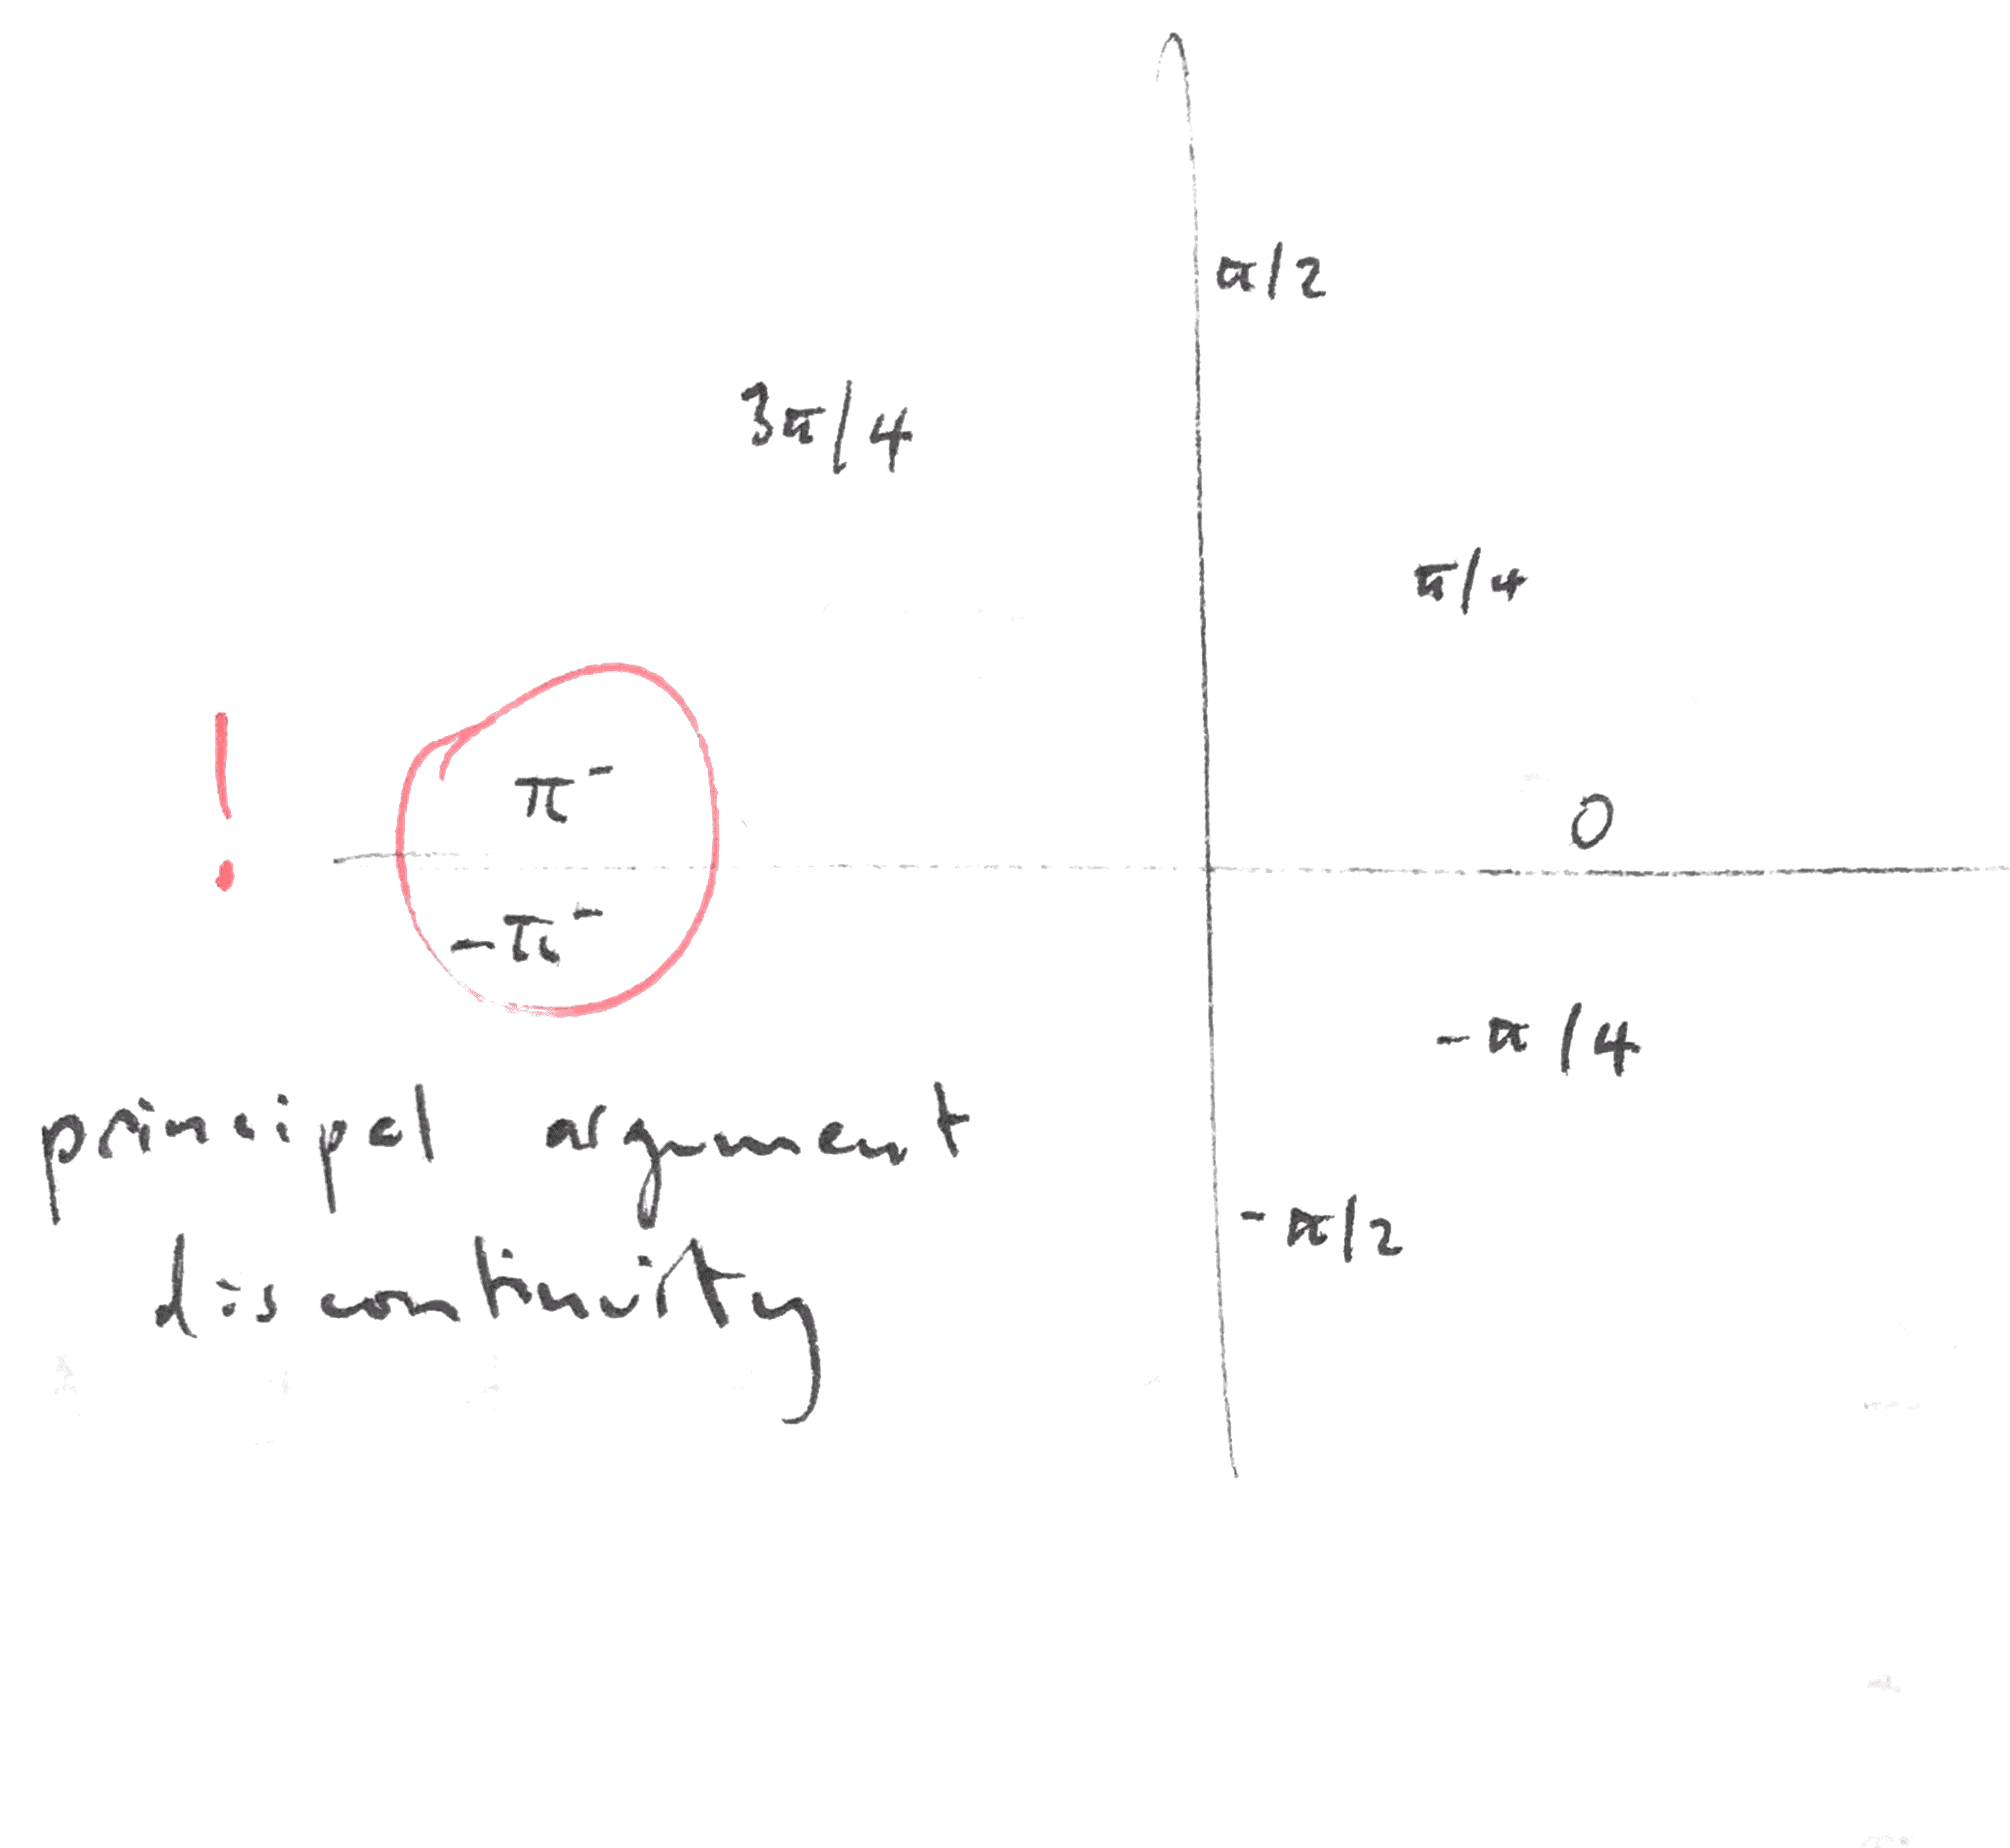
\includegraphics[width=200pt]{img/principal-arg.png}

% The $n$-th roots of $z$ are
% \begin{align*}
%   \sqrt[n] {|z|}\left(\cos\left(\frac{\Arg z + 2k\pi}{n}\right) + i\sin\left(\frac{\Arg z + 2k\pi}{n}\right)\right),
% \end{align*}
% $k = 0, 1, \ldots, n-1$.
% The ``principal root'' is given by $k = 0$:
% \begin{align*}
%   \sqrt[n] {|z|}\left(\cos\frac{\Arg z}{n} + i\sin\frac{\Arg z}{n}\right).
% \end{align*}

% The ``principal branch'' of the log function is given by
% \begin{align*}
%   \Log z = \ln |z| + i\Arg z.
% \end{align*}

% Because they involve $\Arg$, both $\Log$ and the principal root function are
% continuous at points away from the negative real axis.

% Here are some diagrams of the principal branch of the square root
% function. Notice that it is discontinuous at points of the negative real
% axis. I.e. it is a branch in the domain $\C \backslash [0, -\infty)$

% 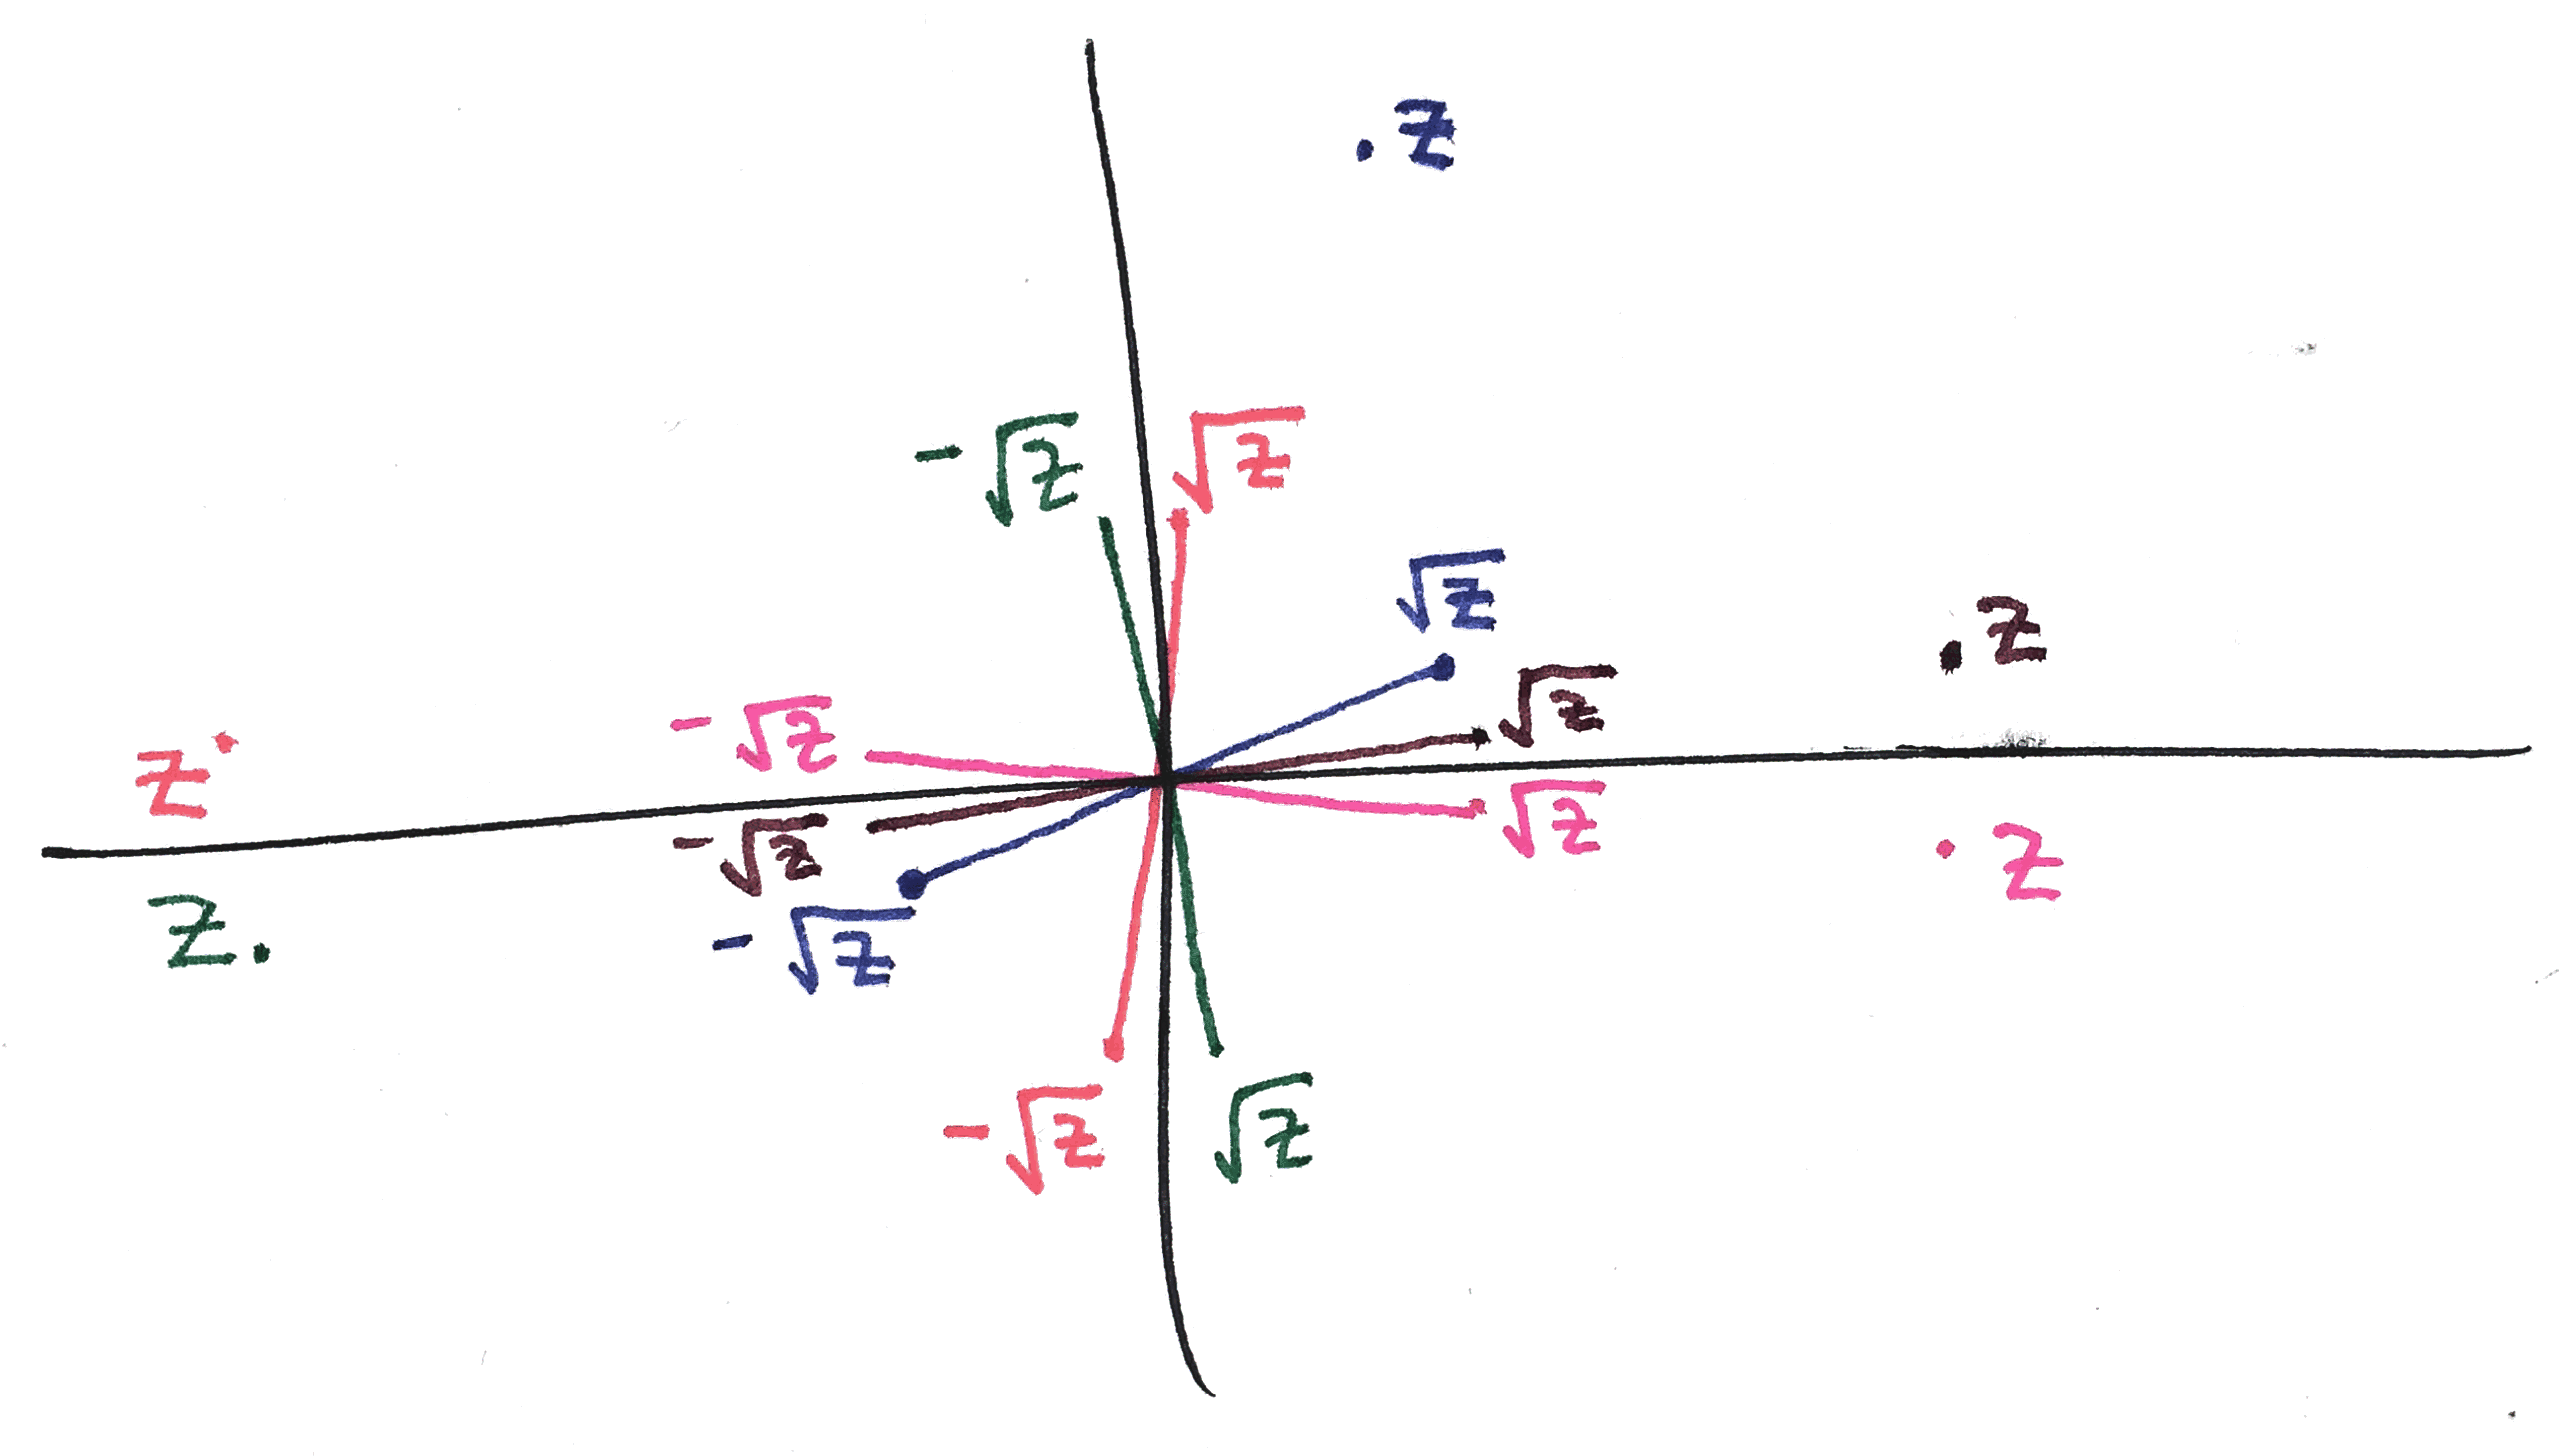
\includegraphics[width=300pt]{img/principal-sqrt-2.png}
% 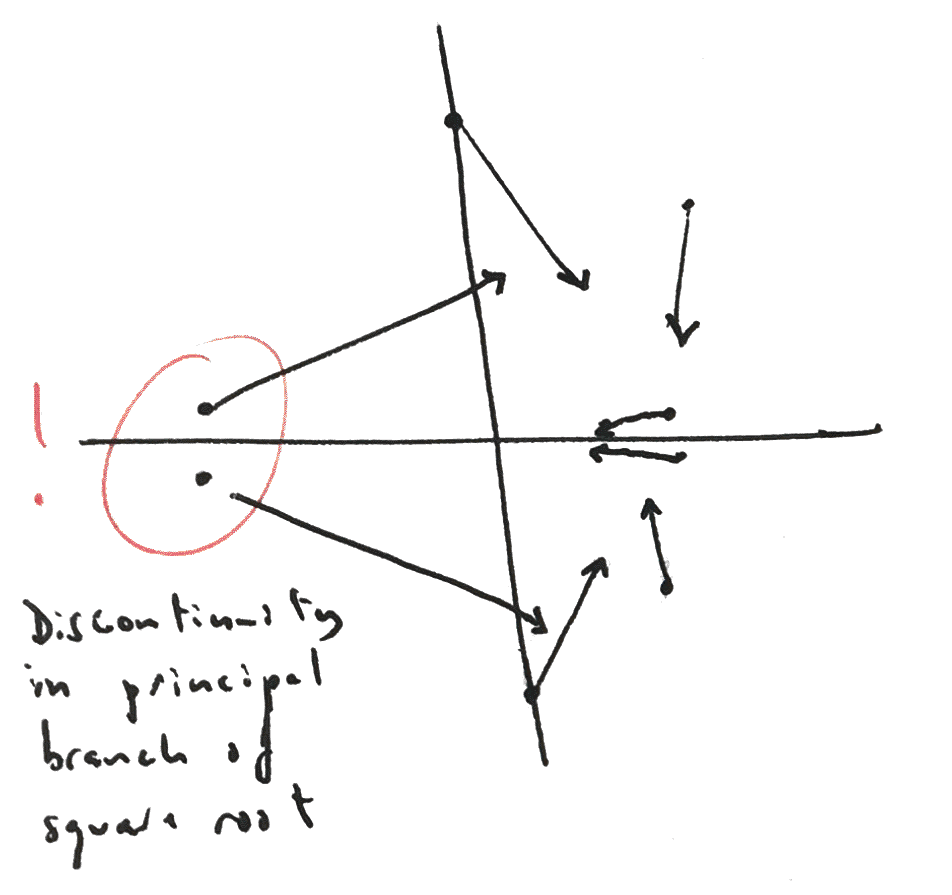
\includegraphics[width=200pt]{img/principal-sqrt.png}

% Suppose we want a branch in a domain that includes the negative real axis. Then we can use
% \begin{align*}
%   g(z) =
%   \begin{cases}
%     \sqrt z,  &\Im z \geq 0\\
%     -\sqrt z, &\Im z < 0
%   \end{cases}
% \end{align*}
% and we could also use $-g$; there are two branches. However, these are
% discontinuous at points on the positive real axis, so they are branches in the
% domain $\C \backslash [0, +\infty)$.

% Consider the infinitely wide strip $\{z: -\pi < \Im z < \pi\}$. The image of
% this under the exponential map is the entire complex plane with 0 removed. For
% example, consider some complex number $w$ with $|w| = r > 0$. It is hit by a
% point on the vertical line $x = \ln r$. So this domain-restricted version of
% the exponential map has an inverse, and that inverse is $\Log$.

% For a multivalent function, it's not possible to find an inverse that sends
% every image point $f(z)$ back to the correct place $z$ on the left-hand side,
% for all $z$. That's because many $z$ hit the same $f(z)$. But it is possible to
% find a ``right inverse'': a function that sends image points back to one of the
% possible preimage points. We want this to be continuous, so we often have to
% restrict the domain on the right-hand side to avoid points of discontinuity,
% e.g. remove $(-\infty, 0]$ in the case of the $\Log$ and principal root inverse
% functions.

% \subsection*{Hyperbolic functions}

% Just as their real counterparts,
% \begin{align*}
%   \cosh z &= (e^z + e^{-z})/2\\
%   \sinh z &= (e^z - e^{-z})/2
% \end{align*}
% with
% \begin{align*}
%   \tanh &= \sinh/\cosh\\
%   \coth &= 1/\tanh\\
%   \sech &= 1/\cosh\\
%   \cosech &= 1/\sinh
% \end{align*}

% \subsection*{Trigonometric functions}

% From $e^{iy} = \cos y + i \sin y$ we have $e^{-iy} = \cos y - i \sin y$ and therefore
% \begin{align*}
%   \cos y &= (e^{iy} + e^{-iy})/2\\
%   \sin y &= (e^{iy} - e^{-iy})/2i,
% \end{align*}
% for real $y$. $\cos$ and $\sin$ are defined on $\C$ by substituting a complex
% variable $z$ in place of $y$:
% \begin{align*}
%   \cos z &= (e^{iz} + e^{-iz})/2\\
%   \sin z &= (e^{iz} - e^{-iz})/2i,
% \end{align*}
% with $\tan, \cot, \sec$ and $\cosec$ also defined as usual.




% \begin{description}
% \exercise{IV.5.2}{
% Describe the curves $|f| = $ constant and $\arg f =$ constant for the function
% \begin{align*}
%   f(z) = \exp(z^2).
% \end{align*}
% }
% Let $z = x + iy$, so
% \begin{align*}
%   f(z)
%   &= \exp((x^2 - y^2) + 2ixy) \\
%   &= e^{x^2 - y^2}\(\cos 2xy + i\sin 2xy\)
% \end{align*}
% % Therefore the set of points $z = x + iy$ for which $|f(z)| = k \in \R$ are
% % those satisfying $e^{x^2 - y^2} = k$.

% Therefore $|f| = k$ for some constant $k \in \R$ implies that
% $e^{x^2 - y^2} = k > 0$, i.e. $y = \pm \sqrt{x^2 - \log k}$. In other words,
% the preimage of a circle of radius $k$ centered on the origin is the union of
% the two curves $y = \pm \sqrt{x^2 - \log k}$.

% $\arg f = \theta$ for some constant $0 \leq \theta < 2\pi$ implies that
% $2xy = \theta$, i.e. $y = \frac{\theta}{2x}$. In other words, the preimage of a
% ray at angle $\theta$ is the graph of $y = \frac{\theta}{2x}$.

% \exercise{IV.9.2}{
%   Find all values of $\log(\log i)$
% } \\\\
% $\log i$ is the following set of image points lying on the imaginary axis:
% \begin{align*}
%   \log i = \left\{i\(\frac{\pi}{2} + 2\pi k\):k \in \Z\right\}.
% \end{align*}
% Fix a particular $k$. The log of the corresponding image point is the following
% set of secondary image points, lying on the vertical line through
% $\frac{\pi}{2} + 2\pi k$:
% \begin{align*}
%   \log \(i\(\frac{\pi}{2} + 2\pi k\)\) = \left\{\log \(\frac{\pi}{2} + 2\pi k\) + i\(\frac{\pi}{2} + 2\pi l\):l \in \Z\right\},
% \end{align*}
% Therefore the set of all values of $\log(\log i)$ is the following rectangular grid of points
% \begin{align*}
%   \log \(\log i\) = \left\{\log \(\frac{\pi}{2} + 2\pi k\) + i\(\frac{\pi}{2} + 2\pi l\):k \in \Z, l \in \Z\right\}.
% \end{align*}

% \exercise{IV.13.3}{
%   [Not in homework.] Let $G$ be the open set one obtains by removing from $\C$
%   the interval $[-1, 1]$ on the real axis. Prove that there is a branch of the
%   function $\sqrt{\frac{z+1}{z-1}}$ in G. (Suggestion: What is the image of $G$
%   under the map $z \mapsto \frac{z+1}{z-1}$?)
% } \\
% The map $z \mapsto \frac{z+1}{z-1}$ maps points as follows:
% \begin{align*}
%   -1 &\mapsto 0  \\
%   0 &\mapsto -1  \\
%   1 &\mapsto \infty \\
%   i &\mapsto -i \\
%   -i &\mapsto i \\
% \end{align*}
% Thus
% \begin{enumerate}
% \item the image of $G$ is $\C$ with the negative real axis removed;
% \item the image of the unit circle is the imaginary axis;
% \item the image of the unit disc is the left half-plane and the image of the
%   complement of the unit disc is the right half-plane.
% \end{enumerate}


% \exercise{IV.13.4}{ Let $G$ be as in Exercise IV.13.3. Prove that there is a
%   branch of the function $\sqrt{z^2 - 1}$ in $G$.
% } \\\\
% Let $f(z) = \sqrt{z^2 - 1}$, using the principal square root function defined by
% \begin{align*}
%   \sqrt w = \sqrt{|w|}\left(\cos\frac{\Arg w}{2} + i\sin\frac{\Arg w}{2}\right).
% \end{align*}
% The principal square root function is discontinuous at points $w$ in
% $(-\infty, 0]$. Therefore $f$ will be continuous for all $z \in \C$ except
% where $z^2 - 1 \in (-\infty, 0]$, i.e.  $-1 \leq z \leq 1$. Therefore $f$ will
% be continuous in $G = \C \backslash [-1, 1]$.


% % A branch of the function $\sqrt{z^2 - 1}$ in $G$ is a function $\phi$ such that
% % for every $z \in G$, $\sqrt{\phi(z)^2 + 1} = z$.

% % Let $f$ be the map $z \mapsto z^2 - 1$.


% $f$ maps points as follows:
% \begin{align*}
%   -1 &\mapsto 0  \\
%   0 &\mapsto -1  \\
%   1 &\mapsto 0 \\
%   i &\mapsto -2 \\
%   -i &\mapsto -2 \\
%   \infty &\mapsto \infty \\
% \end{align*}
% Therefore the image of $G$ under $f$ is $\C$ with the interval $[-1, 0]$ removed.

% % Suppose $f(z) = \sqrt[2^*]{z^2 - 1}$ where $\sqrt[2^*] w$ is the square root of
% % $w$ with smallest positive argument. Then $f$ is not continuous in $G$ since if
% % we travel round the excised interval, the root has changed sign by the time we
% % return to the starting point. So $f$ is not a branch in $G$.

% \exercise{IV.16.1}{
% Find all the values of $(1 + i)^i$.
% } \\\\
% $(1 + i)^i$ is the set of values
% \begin{align*}
%   \exp\left( i\log (1 + i) \right)
%   &= \exp\left(i\left(\log\sqrt 2 + i\left(\frac{\pi}{4} + 2\pi k\right)\right)\right) \\
%   &= \exp\(- \pi\left(2k + \frac{1}{4}\right) + i\frac{\log 2}{2}\) \\
%   &= e^{- \pi\left(2k + \frac{1}{4}\right)}\left(\cos\frac{\log 2}{2} + i\sin\frac{\log 2}{2}\right)
% \end{align*}
% for $k \in \Z$.

% \exercise{IV.16.3}{ Prove that if $f$ is a branch of $z^c$ in an open set not
%   containing 0, then $f$ is holomorphic and $f'$ is a branch of $cz^{c-1}$.
% } \\\\
% A branch $f$ of $z^c$, defined on some open set excluding $0$, means that
% $f(z) = e^{c\Log z}$ for some branch $\Log$ of the logarithm map.

% % Similarly, a branch $g$ of $cz^{c-1}$, defined on the same open set excluding
% % $0$, means that $g(z) = ce^{(c-1)\Log z}$.

% The branch of the logarithm, the exponential function, and multiplication by a
% complex number are all holomorphic transformations. Therefore $f$ is
% holomorphic, because the composition of holomorphic functions with compatible
% domains and ranges is holomorphic.

% The derivative of $f$ is, by the chain rule,
% \begin{align*}
% f'(z) = c e^{c\Log z} \frac{d\Log z}{dz} = c e^{c\Log z} \frac{1}{z} = c \frac{f(z)}{z},
% \end{align*}
% where I have assumed without proof that $\frac{d\Log z}{dz} = \frac{1}{z}$. The
% final expression above is a branch of $cz^{c-1}$ defined in the same region
% that $f$ is defined.

% \end{description}

\section{Power Series}

\begin{description}

  \exercise{V.6.2}{ Prove that the sequence $(g_n)_{n=0}^\infty$ converges
    locally uniformly in the open set $G$ if and only if it converges uniformly
    on each compact subset of $G$.
  }
  \\\\
  First, terminology: Sarason states that $(g_n)_{n=0}^\infty$ converges
  locally uniformly in $G$ if each point of $G$ has a neighborhood in which the
  sequence converges uniformly. I'm going to take that to mean ``if and only if''.

  For the forward direction, we need to show that if

  \emph{(A): each point of $G$ has a neighborhood in which $(g_n)$ converges uniformly}

  then

  \emph{(B): $(g_n)$ converges uniformly on each compact subset of $G$.}

  I don't have a proof, but a suggested approach for how to prove this is by contradiction:
  \begin{enumerate}
  \item Suppose (A) is true but that (B) is not, so that there exists some
    compact subset $S$ of $G$ on which $(g_n)$ does not converge uniformly.
  \item Show that there exists a point of $S$ which lacks any neighborhood
    within which convergence is uniform. $\qed$
  \end{enumerate}

  For the reverse direction, we need to show that if

  \emph{(B): $(g_n)$ converges uniformly on each compact subset of $G$.}

  then

  \emph{(A): each point of $G$ has a neighborhood in which $(g_n)$ converges uniformly}

  Again I don't have a proof, but a suggested approach for how to prove this is:
  \begin{enumerate}
  \item Consider a point $z$ of $G$.
  \item Show that there is a compact subset $S$ of $G$ that contains $z$.
  \item Show that $z$ has a neighborhood which is a subset of $S$. $\qed$
  \end{enumerate}

\exercise{V.7.2}{
  Prove that the series
  $\sum_{n=0}^\infty \(\frac{z-1}{z+1}\)^n$ converges locally uniformly in the
  half-plane $\Re z > 0$, and find the sum.
}

\exercise{V.14.1(b)}{
  Find the radius of convergence of the following series:
  $$
  \sum_{n=0}^\infty \frac{(n!)^3}{(3n)!} z^{3n}
  $$
}
\\\\
We use the ratio test:
\begin{align*}
  \limn \left|\frac{a_n}{a_{n+1}}\right|
  &= \limn \left|\frac{(n!)^3z^{3n}}{(3n)!}
                 \frac{(3n + 3)!}{((n+1)!)^3z^{3n + 3}}\right| \\
  &= |z^{-3}|\limn \left|\frac{(3n + 3)(3n + 2)(3n + 1)}{(n+1)^3}\right| \\
  &= |z^{-3}|\limn \left|\frac{27 + o(n^{-1})}{1 + o(n^{-1})}\right| \\
  &= 27|z^{-3}|
\end{align*}

So the series converges when $|z^3| > 27$, i.e. outside a disc of radius 3
centered at the origin. The radius of convergence is infinite.

\exercise{V.16.2}{
  What function is represented by the power series
  $\sum_{n=1}^\infty n^2z^n$?
}

\exercise{V.18.1}{
  Use the scheme above to determine the power series with center 0 representing
  the function $f(z) = \frac{1}{1 + z + z^2}$ near 0. What is the radius of
  convergence of this series?
}\\\\

Assume $f(z)$ can be represented as a power series $\sum_{n=0}^\infty a_nz^n$. We
can write $f$ as the ratio
\begin{align*}
  f(z) = \frac{1}{1 + z + z^2} = \frac{\sum_{n=0}^0 z^n}{\sum_{n=0}^2 z^n} =: \frac{g(z)}{h(z)}.
\end{align*}

As an infinite power series,
$h(z) = \sum_{n=0}^2 z^n = \sum_{n=0}^\infty b_nz^n$, where $b_n = 1$ for
$0 \leq n \leq 2$ and $b_n$ = 0 otherwise.

Then
\begin{align*}
  g(z) = \sum_{n=0}^0 z^n
  &= f(z)h(z) \\
  &= \(\sum_{n=0}^\infty a_nz^n\)\(\sum_{n=0}^\infty b_nz^n\) \\
  &= \sum_{n=0}^\infty z^n \sum_{k=0}^n a_kb_{n-k} \\
  &= \sum_{n=0}^2 z^n \sum_{k=0}^n a_k \\
  &= a_0 + z(a_0 + a_1) + z^2(a_0 + a_1 + a_2)
\end{align*}
\end{description}
Therefore $a_0 = 1$, $a_1 = -a_0 = -1$ and $a_2 = 0$, so
\begin{align*}
  f(z) = 1 - z
\end{align*}

\end{document}
